\documentclass[12pt]{report}
\usepackage[numbers]{natbib}
\bibliographystyle{unsrtnat}

\usepackage{amssymb}

\usepackage{hyperref}
\usepackage{cleveref}
\usepackage{xspace}

\usepackage{graphicx} % Required for inserting images
\usepackage{geometry}
\geometry{margin=1in}
\usepackage{subcaption}
\usepackage{listings}
\usepackage{xcolor}
\usepackage[parfill]{parskip}

\definecolor{codegreen}{rgb}{0,0.6,0}
\definecolor{codegray}{rgb}{0.5,0.5,0.5}
\definecolor{codepurple}{rgb}{0.58,0,0.82}
\definecolor{backcolour}{rgb}{0.95,0.95,0.92}

\lstdefinestyle{mystyle}{
    backgroundcolor=\color{backcolour},   
    commentstyle=\color{codegreen},
    keywordstyle=\color{magenta},
    numberstyle=\tiny\color{codegray},
    stringstyle=\color{codepurple},
    basicstyle=\ttfamily\footnotesize,
    breakatwhitespace=false,         
    breaklines=true,                 
    captionpos=b,                    
    keepspaces=true,                 
    numbers=left,                    
    numbersep=5pt,                  
    showspaces=false,                
    showstringspaces=false,
    showtabs=false,                  
    tabsize=2
}

\lstset{style=mystyle}

\usepackage[T1]{fontenc}
\usepackage{tgbonum}

\def\libspataud{\texttt{libspatialaudio}\xspace}
\def\deg{$^{\circ}$ }
\newcommand{\code}[1]{\texttt{#1}}

\title{\libspataud: Spatial Audio Library for Ambisonic, Object, Speaker and Binaural Rendering}
\author{Peter Stitt}
\date{October 2025}

\makeatletter
\let\newtitle\@title
\let\newauthor\@author
\let\newdate\@date
\makeatother

\begin{document}

\maketitle

\tableofcontents

\chapter{Getting Started}\label{GettingStarted}

\section{Introduction}
% Summarise what it does and what is its intended purpose. What are the stages of its evolution?
\libspataud\footnote{\href{https://github.com/videolabs/libspatialaudio}{https://github.com/videolabs/libspatialaudio}} is an open source library for rendering spatial audio.
Originally it is a fork of ambisonic-lib from Aristotel Digenis.
It was adopted and extended for spatial audio rendering in VLC Media Player 3.0\footnote{\href{https://www.videolan.org/vlc/releases/3.0.20.html}{https://www.videolan.org/vlc/releases/3.0.20.html} Last accessed 20/11/2023} in 2017 and further extended in 2020 to incorporate a renderer compatible with Audio Definition Model (ADM) streams \cite{ITU2076}, based on the ADM renderer specification ITU-R BS.2127 \cite{ITU2127}. This extension added DirectSpeaker and Object rendering to the library.

The library can be used to encode mono signals to Ambisonics, to decode Ambisonics to loudspeakers or to binaural.
It can also perform sound field rotations, which allows it to be used with data from a head-tracker.
The main spatialisation processors are outlined in \cref{Ambisonics}, along with the theoretical background on which they are based.
\libspataud also includes a renderer that allows it to use metadata to spatialise an audio stream.
The renderer can accept Object, HOA and DirectSpeaker streams and can render to loudspeakers or binaural.
It can be used for rendering ADM or IAMF signals.
Chapter \ref{Renderer} outlines the \libspataud Renderer (compatible with ADM ITU-R BS.2127 and IAMF).
Code examples are given for those interested primarily in implementation of \libspataud.

The library allows you to encode, decode, rotate, zoom HOA audio streams up to the 3rd order. It can output to standard and custom loudspeakers arrays. To playback with headphones, the binauralizer applies an HRTF (either a SOFA file or  the included MIT HRTF) to provide a spatial binaural rendering effect. The binauralization can also be used to render multichannel streams (5.1, 7.1...).

\section{Features}

The library has four main uses:
\begin{itemize}
    \item Ambisonics: encoding, rotation, zooming, psychoacoustic optimisation and decoding of HOA signals is provided. These function up to 3rd order Ambisonics. For more details on the Ambisonics capabilities of \libspataud please see \cref{Ambisonics}.
    \item Loudspeaker Binauralization: convert loudspeaker signals to binaural, with the option to use custom HRTFs loaded via a SOFA file. Read more on how to binauralise loudspeaker signals \cref{Binauralization}.
    \item Object Spatialisation: convert mono signals to loudspeaker signals. The sound source is panned as a point source using amplitude panning. For a guide on how to spatialise objects please see \cref{ObjectSpatialisation}.
    \item Metadata-based Renderering: render Object, DirectSpeaker, HOA and Binaural streams using their metadata based on Rec. ITU-R BS.2127-1. For a guide on how to use the Renderer see \cref{Renderer}.
\end{itemize}

\section{Learning About \libspataud}

The documentation includes
\begin{itemize}
\item background theory (mathematical, psychoacoustic, DSP).
\begin{itemize}
\item All background theory sections have been written such that it should be accessible to anyone with some mathematical background.
However, even without a mathematical background you should still be able to follow what is going on.
\end{itemize}
\item implementation details (layout out the choices made while writing the library)
\item code examples (overviews of the main classes and code examples).
\end{itemize}

To learn more about the Ambisonics processors start in \cref{Ambisonics}.
To learn more about the Renderer start in \cref{Renderer}.
These two chapters provide full examples of both signal flows, as well as links to more details for those who want to learn more or get more specific details.

For those who do not need to know the background theory, most sections contain details of the code, as well as an example of how to implement it separately from the theory.

\section{Building \libspataud}

To build \libspataud, follow these steps:
\begin{enumerate}
    \item 1. Clone the repository (if you haven't already):
\begin{lstlisting}[language=bash]
    git clone https://github.com/videolabs/libspatialaudio.git
    cd libspatialaudio
\end{lstlisting}
\item  Create a `build` directory and navigate into it:
\begin{lstlisting}[language=bash]
    mkdir build
    cd build
\end{lstlisting}
\item Run CMake to configure the project:
\begin{lstlisting}[language=bash]
    cmake ..
\end{lstlisting}
\item Build the project using Make:
\begin{lstlisting}[language=bash]
    make
\end{lstlisting}
\end{enumerate}

\section{License}

libspatialaudio is released under LGPLv2.1 (or later) and is also available
under a commercial license. For full details see \href{https://github.com/videolabs/libspatialaudio/blob/master/LICENSE}{the LICENSE file}.

\chapter{Ambisonic Processing}\label{Ambisonics}

\section{Overview of Ambisonic Processors}\label{AmbisonicOverview}

\subsection{Ambisonic Processors}

The main Ambisonic processing classes are:
\begin{itemize}
\item \code{AmbisonicEncoder}: Converts a mono signal to an Ambisonics signal of order 1 to 3. Read more in \cref{AmbiEncoding}.
\item \code{AmbisonicRotator}: Applies a user-specified rotation to the sound field. This is useful for head tracking or keeping the audio aligned with a 360 video. Read more in \cref{AmbiRotation}.
\item \code{AmbisonicZoomer}: An acoustical "zoom" that focuses on the front of the sound scene. Read more in \cref{AmbiZoomer}.
\item \code{AmbisonicDecoder}: A decoder that converts an Ambisonics signal to a set of loudspeaker signals. It contains optimised presets for 5.1 and 7.1 loudspeaker layouts. Custom layouts can also have their decoding matrix defined by the user, for additional flexibility. Read more in \cref{AmbisonicDecoder}.
\item \code{AmbisonicBinauralizer}: A decoder that converts an Ambisonics signal to a binaural signal. This allows for immersive audio to be experienced over headphones. Custom HRTFs can be loaded using the .SOFA format, allowing for a customised listening experience. Read more in \cref{AmbiToBin}.
\item \code{AmbisonicAllRAD}: A decoder that converts an Ambisonics signal to a set of loudspeaker signals corresponding to the ITU layouts or IAMF specificiation layouts. It uses the AllRAD method to calculate the decoding matrix. Read more in \cref{AmbisonicAllRAD}.
\end{itemize}

\subsection{Ambisonics Signal Flow}

In general, unless your signal is already in Ambisonics format, the signal chain will begin with \code{AmbisonicEncoder} to bring the audio in to the Ambisonics domain.
The rotation and zooming processing elements are optional and will be context dependent. However, they should generally be applied to a summation of all the sound sources making up the scene, rather than applying to each one individually.

Finally, the signal needs to be converted from a Ambisonics to the listener's particular layout. The choice of which decoder should be used is generally decided by the target output layout. ITU layouts could use \code{AmbisonicAllRAD} or, if a custom decoder is available, \code{AmbisonicDecoder}. Binauralisation over headphones uses \code{AmbisonicBinauralization}.

\begin{figure}
    \centering
    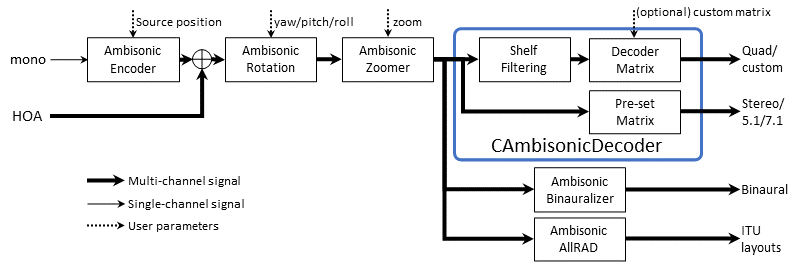
\includegraphics[width = \textwidth]{figures/AmbisonicSignalFlow.png}
    \caption{The signal flow to encode a mono signal to HOA, adding to any pre-encoded HOA streams, with rotation and zooming processing before decoding to different formats.}
    \label{fig:ambi_signal_flow}
\end{figure}

The above figure shows the signal flow used to encode a mono input signal to HOA, perform rotation of the sound field (using \code{AmbisonicRotator}) and then to acoustically zoom on the front of the sound field (using \code{AmbisonicZoomer}).
Finally, it is decoded to the listener using one of the decoding methods.

\subsection{Code Example}

This example shows how to apply the entire signal chain described above and to convert the output to binaural.

See [here](AmbisonicDecoding.md) for specific examples on how to decode using `AmbisonicDecoder` or `AmbisonicAllRAD`.

\begin{lstlisting}[language=C++]
#include "Ambisonics.h"

using namespace spaudio;

const unsigned int sampleRate = 48000;
const int nBlockLength = 512;

// Higher ambisonic order means higher spatial resolution and more channels required
const unsigned int nOrder = 1;
// Set the fade time to the length of one block
const float fadeTimeInMilliSec = 1000.f * (float)nBlockLength / (float)sampleRate;

std::vector<float> sinewave(nBlockLength);
// Fill the vector with a sine wave
for (int i = 0; i < nBlockLength; ++i)
    sinewave[i] = (float)std::sin((float)M_PI * 2.f * 440.f * (float)i / (float)sampleRate);

// B-format buffer
BFormat myBFormat;
myBFormat.Configure(nOrder, true, nBlockLength);
myBFormat.Reset();

// Encode the signal to Ambisonics
AmbisonicEncoder myEncoder;
myEncoder.Configure(nOrder, true, sampleRate, 0);
PolarPosition<float> position;
position.azimuth = 0;
position.elevation = 0;
position.distance = 1.f;
myEncoder.SetPosition(position);
myEncoder.Reset();

// Set up the rotator
AmbisonicRotator myRotator;
myRotator.Configure(nOrder, true, nBlockLength, sampleRate, fadeTimeInMilliSec);
RotationOrientation rotOri;
rotOri.yaw = 0.5 * M_PI;
myRotator.SetOrientation(rotOri);

// Set up the zoomer processor
AmbisonicZoomer myZoomer;
myZoomer.Configure(nOrder, true, nBlockLength, 0);
myZoomer.SetZoom(0.5f);

// Set up the binaural decoder
AmbisonicBinauralizer myDecoder;
unsigned int tailLength = 0;
myDecoder.Configure(nOrder, true, sampleRate, nBlockLength, tailLength);
// Configure buffers to hold the decoded signal
const unsigned int nEar = 2;
float** earOut = new float* [nEar];
for (int iEar = 0; iEar < nEar; ++iEar)
    earOut[iEar] = new float[nBlockLength];

// Process the audio ==============================
// Encode the signal to Ambisonics
myEncoder.Process(sinewave.data(), nBlockLength, &myBFormat);

// Rotate the Ambisonics signal
myRotator.Process(&myBFormat, nBlockLength);

// Apply zooming to the Ambisonics signal
myZoomer.Process(&myBFormat, nBlockLength);

// Decode the signal to binaural
myDecoder.Process(&myBFormat, earOut, nBlockLength);

// Cleanup
for (unsigned iEar = 0; iEar < nEar; ++iEar)
    delete[] earOut[iEar];
delete[] earOut;
\end{lstlisting}

\section{Ambisonic Encoding}\label{AmbiEncoding}

\subsection{Theory and Implementation Details}
Ambisonic encoding is the conversion of a mono signal to Ambisonics of a specified order.
Ambisonic order governs the spatial resolution of the sound scene.
Higher orders lead to higher resolution at the expense of increased processing requirements.
The number of encoded channels is $(N + 1)^{2}$ meaning 1st, 2nd and 3rd order require 4, 9 and 16 channels respectively.

A mono input signal is converted to Ambisonics through multiplication with a series of encoding gains.
\libspataud uses the AmbiX specification \cite{nachbar_ambix_2011}, which orders the channels in the ACN format and uses SN3D normalisation.
The encoded signal is thus calculated as
\begin{equation}
    \textbf{b}_{N}(t) = \textbf{y}_{N}(\theta,\phi)s(t)
\end{equation}
\sloppy where $s(t)$ is the mono input signal at time $t$ and $\textbf{y}_{N}(\theta,\phi)$ is a column vector of length $(N + 1)^{2}$ containing the SN3D-weighted spherical harmonic gains $[Y_{0}^{0}(\theta, \phi), Y_{1}^{-1}(\theta, \phi), Y_{1}^{0}(\theta, \phi),\ldots,Y_{N}^{N}(\theta, \phi)]^{\mathrm{T}}$. The angles $\theta$ and $\phi$ are the direction of the sound source and are expected in degrees. The azimuth $\theta$ is positive in the anti-clockwise direction, so +90\deg is to the left of the listener. The elevation $\phi$ ranges from -90\deg below the listener to +90\deg above.

\subsubsection{Encoding Gain Interpolation}

In order to allow to real-time changes in source direction with minimal audio artefacts ("zipper" sounds) as the direction changes, \code{AmbisonicEncoder} uses an instance of \code{GainInterp} internally.
Every time the direction of the source is changed the gain vector $\textbf{y}_{N}(\theta,\phi)$ is updated and a linear interpolation is applied going from the current to new values.
This length of the interpolation can be specified by the user.
Its ideal length will depend on the signals but 10 ms will reduce most "zipper" sounds.

\subsection{\code{AmbisonicEncoder}}

The \code{AmbisonicEncoder} class is used to convert a mono signal to Ambisonics. When the encoding position is modified it internally smooths the encoding gains $\textbf{y}_{N}(\theta,\phi)$ to avoid unwanted clicks in the output.

\subsubsection{Configuration}

Before calling any other functions the object must first be configured by calling \code{Configure()} with the appropriate values. If the values are supported then the it will return `true` and the object can now be used.

The configuration parameters are:
\begin{itemize}
    \item nOrder: The ambisonic order from 1 to 3.
    \item b3D: A bool to indicate if the signal is to be encoded to 2D (azimuth only) or 3D (azimuth and elevation). 3D should be preferred.
    \item sampleRate: The sample rate of the audio being used e.g. 44100 Hz, 48000 Hz etc. This must be an integer value greater than zero.
    \item fadeTimeMilliSec: The time in milliseconds to fade from an old set of encoding gains to another. Lower values will lead to lower latency at the expense of possible audio artefacts. Higher values will lead to increased latency before the source reaches the new encoded position. A value of 10 ms is usually a good starting point.
\end{itemize}

\subsubsection{Set Encoding Direction}

The encoding direction is set as a polar direction in radians using the \code{SetPosition()} function. It takes a \code{PolarPosition<float>} as an input.

Note: the distance is ignored. Only the encoding direction is set.

\subsubsection{Encoding a Signal}

An array of floats can be encoded using either the \code{Process()} or \code{ProcessAccumul()} functions. These two functions process the input signal in the same way. The only difference is that \code{ProcessAccumul()} will add the newly encoded signal to the output with an optional gain, whereas \code{Process()} will replace the destination signal with the encoded signal.

The inputs are:
\begin{itemize}
    \item pfSrc: A pointer to the mono input signal.
    \item nSamples: The length of the input signal in samples.
    \item pBFDst: A pointer to the destination B-format signal.
    \item nOffset: Optional offset position when writing to the output. When set to zero this will write the signal to the start of \code{pBFDst}. Any non-zero value will write to the output with a delay of the specified number of samples, leaving any preceding samples unchanged. The offset and input signal length must not be such that the encoded signal would be written beyond the end of \code{pBFDst} i.e. \code{nSamples + nOffset <= pfDst->GetSampleCount()}.
    \item (\code{ProcessAccumul()} only) fGain: Optional gain to apply to the output before it is added to the signal in `pBFDst`.
\end{itemize}

\subsection{Code Example}

This example shows how to convert a mono sine wave to an Ambisonics signal that rotates around the listener from the front and then to the left, back, right and back to the front.

\begin{lstlisting}[language=C++]
#include "Ambisonics.h"

using namespace spaudio;

const unsigned int sampleRate = 48000;
const int nBlockLength = 512;
const int nBlocks = 94;
const int nSigSamples = nBlocks * nBlockLength; // Approximately 1 second @ 48 kHz

// Higher ambisonic order means higher spatial resolution and more channels required
const unsigned int nOrder = 1;
// Set the fade time to the length of one block
const float fadeTimeInMilliSec = 1000.f * (float)nBlockLength / (float)sampleRate;

std::vector<float> sinewave(nSigSamples);
// Fill the vector with a sine wave
for (int i = 0; i < nSigSamples; ++i)
    sinewave[i] = (float)std::sin((float)M_PI * 2.f * 440.f * (float)i / (float)sampleRate);

// Destination B-format buffer
BFormat myBFormat;
myBFormat.Configure(nOrder, true, nSigSamples);
myBFormat.Reset();

// Set up and configure the Ambisonics encoder
AmbisonicEncoder myEncoder;
myEncoder.Configure(nOrder, true, sampleRate, fadeTimeInMilliSec);

// Set test signal's initial direction in the sound field
PolarPosition<float> position;
position.azimuth = 0;
position.elevation = 0;
position.distance = 1.f;
myEncoder.SetPosition(position);
myEncoder.Reset();

for (int iBlock = 0; iBlock < nBlocks; ++iBlock)
{
    // Update the encoding position to reach by the end of the block
    position.azimuth = (float)(iBlock + 1) / (float)nBlocks * 2.f * (float)M_PI;
    myEncoder.SetPosition(position);

    // Encode the first block, writing to the appropriate point of the destination buffer
    const unsigned int iSamp = iBlock * nBlockLength;
    myEncoder.Process(&sinewave[iSamp], nBlockLength, &myBFormat, iSamp);
}
\end{lstlisting}

\section{Ambisonic Rotation}\label{AmbiRotation}

\subsection{Theory and Implementation Details}

Any signal in the ambisonic domain can be rotated by application of a rotation matrix.
This allows (for example) headtracking data to be used to rotate the sound field in the opposite direction to how the listener is moving their head, which will keep the sound sources in the correct position in space, rather than them moving with the listeners head.

Rotation is performed by multiplying the Ambisonic signal $\textbf{b}_{N}(t)$ by a rotation matrix:
\begin{equation}
    \textbf{b}'_{N}(t) = \textbf{R}_{N}(\alpha, \beta, \gamma) \textbf{b}_{N}(t).
\end{equation}

The rotation angles are yaw, pitch and roll around the z-axis, y-axis and x-axis respectively.

A positive yaw angle will cause a sound source to rotated in a clockwise direction with respect to the origin when viewed from along the z-axis (above). From the point-of-view of the listener this is as if they turn to their left.

A positive pitch angle will cause a sound source to move above the listener. From the point-of-view of the listener this is as if they tilt their head forward.

A positive roll angle will rotate a sound from the left to the right underneath the listener. From the point-of-view of the listener this is as if they roll their head to the right.

Rotations can be applied in any order but changing the order of the rotation will not result in the same output, so care must be taken.
The yaw-pitch-roll order, where rotations around the z-axis are performed first, is common in Ambisonics, but \code{AmbisonicRotator} gives the option for any combination to be used.

Rotation of the sound field is particularly beneficial when working with a binaural renderer because it fixes the sound sources in space.
This can help to reduce front-to-back confusions or with sound source externalisation.

Note that \code{AmbisonicRotator} uses hard-coded equations to generate the individual yaw, pitch and roll rotation matrices. However, for higher orders a recurrence relation based method can be used to compute $\textbf{R}_{N}(\alpha, \beta, \gamma)$ \cite{ivanic1996rotation}.

\subsection{\code{AmbisonicRotator}}

The \code{AmbisonicRotator} class is used to change the orientation of a supplied Ambisonic signal in real-time. In order to avoid clicks while rotating the rotation matrices are interpolated over a specified length of time set during configuration of the object.

\subsubsection{Configuration}

Before calling any other functions the object must first be configured by calling \code{Configure()} with the appropriate values. If the values are supported then it will return \code{true} and the object can now be used.

The configuration parameters are:

- \textbf{nOrder}: The ambisonic order from 1 to 3.
- \textbf{b3D}: \code{AmbisonicRotator} only supports rotation of 3D sound scenes. This should be set to \code{true} or else configuration will fail.
- \textbf{nBlockSize}: The maximum block size \code{Process()} is expected to handle.
- \textbf{sampleRate}: The sample rate of the audio being used e.g. 44100 Hz, 48000 Hz etc. This must be an integer value greater than zero.
- \textbf{fadeTimeMilliSec}: The time in milliseconds to fade from an old matrix to another. Lower values will lead to lower latency at the expense of possible audio artefacts. Higher values will lead to increased latency before the source reaches the new orientation. A value of 10 ms is usually a good starting point.

\subsubsection{Set Rotation Order and Orientation}

The default rotation ordering is yaw-pitch-roll. However, any desired order can be specified using \code{SetRotationOrder()}. Changing the rotation ordering will cause the rotation matrix to be updated using the new ordering.

The yaw, pitch, and roll values are set by passing a \code{RotationOrientation} to \code{SetOrientation()}. The rotation angles should be supplied in radians.

\subsubsection{Rotating an Ambisonic Signal}

A B-format signal can be rotated using the \code{Process()} function. The input signal is replaced by the rotated signal. The inputs are:

- \textbf{pBFSrcDst}: A pointer to the source B-format signal that is replaced with the processed signal.
- \textbf{nSamples}: The length of the input signal in samples.

\subsection{Code Example}

This example shows how to rotate an Ambisonics signal by 90\deg ($\pi/2$ radians) so that it is heard as coming from the right of the listener when decoded.

\begin{lstlisting}[language=C++]
#include "Ambisonics.h"

using namespace spaudio;

const unsigned int sampleRate = 48000;
const int nBlockLength = 512;

// Higher ambisonic order means higher spatial resolution and more channels required
const unsigned int nOrder = 1;
// Set the fade time to the length of one block
const float fadeTimeInMilliSec = 1000.f * (float)nBlockLength / (float)sampleRate;

std::vector<float> sinewave(nBlockLength);
// Fill the vector with a sine wave
for (int i = 0; i < nBlockLength; ++i)
    sinewave[i] = (float)std::sin((float)M_PI * 2.f * 440.f * (float)i / (float)sampleRate);

// B-format buffer
BFormat myBFormat;
myBFormat.Configure(nOrder, true, nBlockLength);
myBFormat.Reset();

// Encode the signal to Ambisonics
AmbisonicEncoder myEncoder;
myEncoder.Configure(nOrder, true, sampleRate, 0);
PolarPosition<float> position;
position.azimuth = 0;
position.elevation = 0;
position.distance = 1.f;
myEncoder.SetPosition(position);
myEncoder.Reset();
myEncoder.Process(sinewave.data(), nBlockLength, &myBFormat);

// Set up the rotator
AmbisonicRotator myRotator;
myRotator.Configure(nOrder, true, nBlockLength, sampleRate, fadeTimeInMilliSec);
RotationOrientation rotOri;
rotOri.yaw = 0.5 * M_PI; // pi/2 radians = 90 degrees
myRotator.SetOrientation(rotOri);

// Rotate the Ambisonics signal
myRotator.Process(&myBFormat, nBlockLength);
\end{lstlisting}

\section{Ambisonic Zoomer}\label{AmbiZoomer}
\subsection{Theory and Implementation Details}

The \code{AmbisonicZoomer} class allows for a kind of acoustic zoom to the front of the sound field.
It was implemented for use with the zoom function with 360-videos in VLC Media Player to place emphasis on sounds in the view direction.

It samples the sound field to the front with a virtual cardioid microphone with order matching the order of the input signal.
This mono virtual microphone signal is then re-encoded back to a signal at the front of the sound field and blended with the full sound field based on the zoom value set in \code{AmbisonicZoomer::SetZoom}.

A zoom value of 0 will perform no transformation to the ambisonic signal while a zoom of 1 will lead to an extreme zoom, which results in mono signal encoded to the front of the sound field.

Another method for achieving a similar effect would be to decode the Ambisonics signal to a set of points regularly spaced on the sphere, applying a directional weight to these points, then re-encoding the points to Ambisonics.
However, this requires a transformation from and to the Ambisonics domain over a large number of points. This makes it more CPU intensive than the simple method used here, and so it is not implemented in \code{libspatialaudio}.

\subsection{\code{AmbisonicZoomer}}

\subsubsection{Configuration}

Before calling any other functions the object must first be configured by calling \code{Configure()} with the appropriate values. If the values are supported then it will return \code{true} and the object can now be used.

The configuration parameters are:
\begin{itemize}
    \item \textbf{nOrder}: The ambisonic order from 1 to 3.
    \item \textbf{b3D}: A bool to indicate if the signal to be decoded is 2D (azimuth only) or 3D (azimuth and elevation).
    \item \textbf{nBlockSize}: The maximum block size \code{Process()} is expected to handle.
    \item \textbf{sampleRate}: The sample rate of the signal expected by `Process()`.
\end{itemize}

\subsubsection{Setting the Zoom Amount}

The amount of zoom can be set from 0 to 1 using \code{SetZoom()}. A value of 0 corresponds to no zoom and the signal will be returned unchanged after processing.
A value of 1 means that the maximum amount of zooming will be applied and almost all of the signal will be from the re-encoded forward-facing virtual microphone.

\subsubsection{Zooming a Signal}

A B-format signal can have zooming applied using the \code{Process()} function. The input signal is replaced by the processed signal.

The inputs are:
\begin{itemize}
    \item \textbf{pBFSrcDst}: A pointer to the source B-format signal.
    \item \textbf{nSamples}: The number of samples to process.
\end{itemize}

\subsubsection{Code Example}

This example shows how to apply zooming to an Ambisonics signal.

\begin{lstlisting}[language=C++]
#include "Ambisonics.h"

using namespace spaudio;

const unsigned int sampleRate = 48000;
const int nBlockLength = 512;

// Higher ambisonic order means higher spatial resolution and more channels required
const unsigned int nOrder = 1;

std::vector<float> sinewave(nBlockLength);
// Fill the vector with a sine wave
for (int i = 0; i < nBlockLength; ++i)
    sinewave[i] = (float)std::sin((float)M_PI * 2.f * 440.f * (float)i / (float)sampleRate);

// B-format buffer
BFormat myBFormat;
myBFormat.Configure(nOrder, true, nBlockLength);
myBFormat.Reset();

// Encode the signal to Ambisonics
AmbisonicEncoder myEncoder;
myEncoder.Configure(nOrder, true, sampleRate, 0);
PolarPosition<float> position;
position.azimuth = 0;
position.elevation = 0;
position.distance = 1.f;
myEncoder.SetPosition(position);
myEncoder.Reset();
myEncoder.Process(sinewave.data(), nBlockLength, &myBFormat);

// Set up the zoomer processor
AmbisonicZoomer myZoomer;
myZoomer.Configure(nOrder, true, nBlockLength, 0);
myZoomer.SetZoom(0.5f);

// Apply zooming to the Ambisonics signal
myZoomer.Process(&myBFormat, nBlockLength);
\end{lstlisting}

\section{Ambisonic Psychoacoustic Optimisation}\label{AmbiShelves}

When decoding ambisonic signals to loudspeakers (or binaural using the virtual loudspeaker approach) there is a limit frequency $f_{\mathrm{lim}}$ above which the sound field is no longer considered well-reproduced.
This limit frequency increases with the ambisonic order as can be approximated using \cite{Bertet2013}
\begin{equation}
    f_{\mathrm{lim}} = \frac{c N}{4 R (N + 1) \sin(\pi/(2N + 2))}
\end{equation}
where $c$ is the speed of sound in m/s, and $R$ is the radius of the reproduction area in metres.
For a central listener, and assuming $R = 0.09$~m (approximate radius of a human head), the limit frequencies for first- to third-order are approximately 674~Hz, 1270~Hz, and 1867~Hz.

Ambisonic theory optimises for the velocity vector at low frequencies and the energy vector at higher ones.
This optimision is performed simply by applying a gain by-order to the input signal.
At low frequencies the gain is unity and this is known as a basic decoder.
At higher frequencies the gains are chosen to psychoacoustically optimised the signal.
This is done such that the energy in the decoded loudspeaker array is concentrated in the source direction.
This is known as max $\textbf{r}_{\textrm{E}}$ decoding.

The weights applied to the channels of each set of channels of degree $n$ are
\begin{equation}
a_{n}^{2D} = \cos\left( \frac{n\pi}{2N + 2} \right)\\
\end{equation}
for 2D decoding \cite{Daniel2000}.
For 3D decoding they can be approximated using \cite{Zotter2012a}
\begin{equation}
    a_{n}^{3D} = P_{n}\left(\cos \left(\frac{137.9^{\circ}}{N + 1.51}\right) \right)
\end{equation}
where $P_{n}$ is a Legendre polynomial.
The decoding equation \cref{eqn:decode} becomes
\begin{equation}\label{eqn:optimised_decode}
\textbf{x}(t) = \textbf{D}_{N}^{\mathrm{SN3D}} \mathrm{diag}(\textbf{a}_N)\textbf{b}_{N}(t)
\end{equation}
where $\textbf{a}_N$ is a vector of length $(N + 1)^{2}$ containing the max $r_{\mathrm{E}}$ gains with an energy compensation gain applied.
The gains applied to frequencies below the limit frequency are all unity so $\mathrm{diag}(\textbf{a}_N)$ is the identity matrix, meaning \cref{eqn:optimised_decode} collapses back to \cref{eqn:decode}.

The frequency-dependent application of these gains leads to a set of shelf filters that are applied to channels of the same order.
The filtered signal can then be decoded using a frequency-independent decoder.

\subsubsection{Shelf Filter Implementation}

\begin{figure}
    \centering
    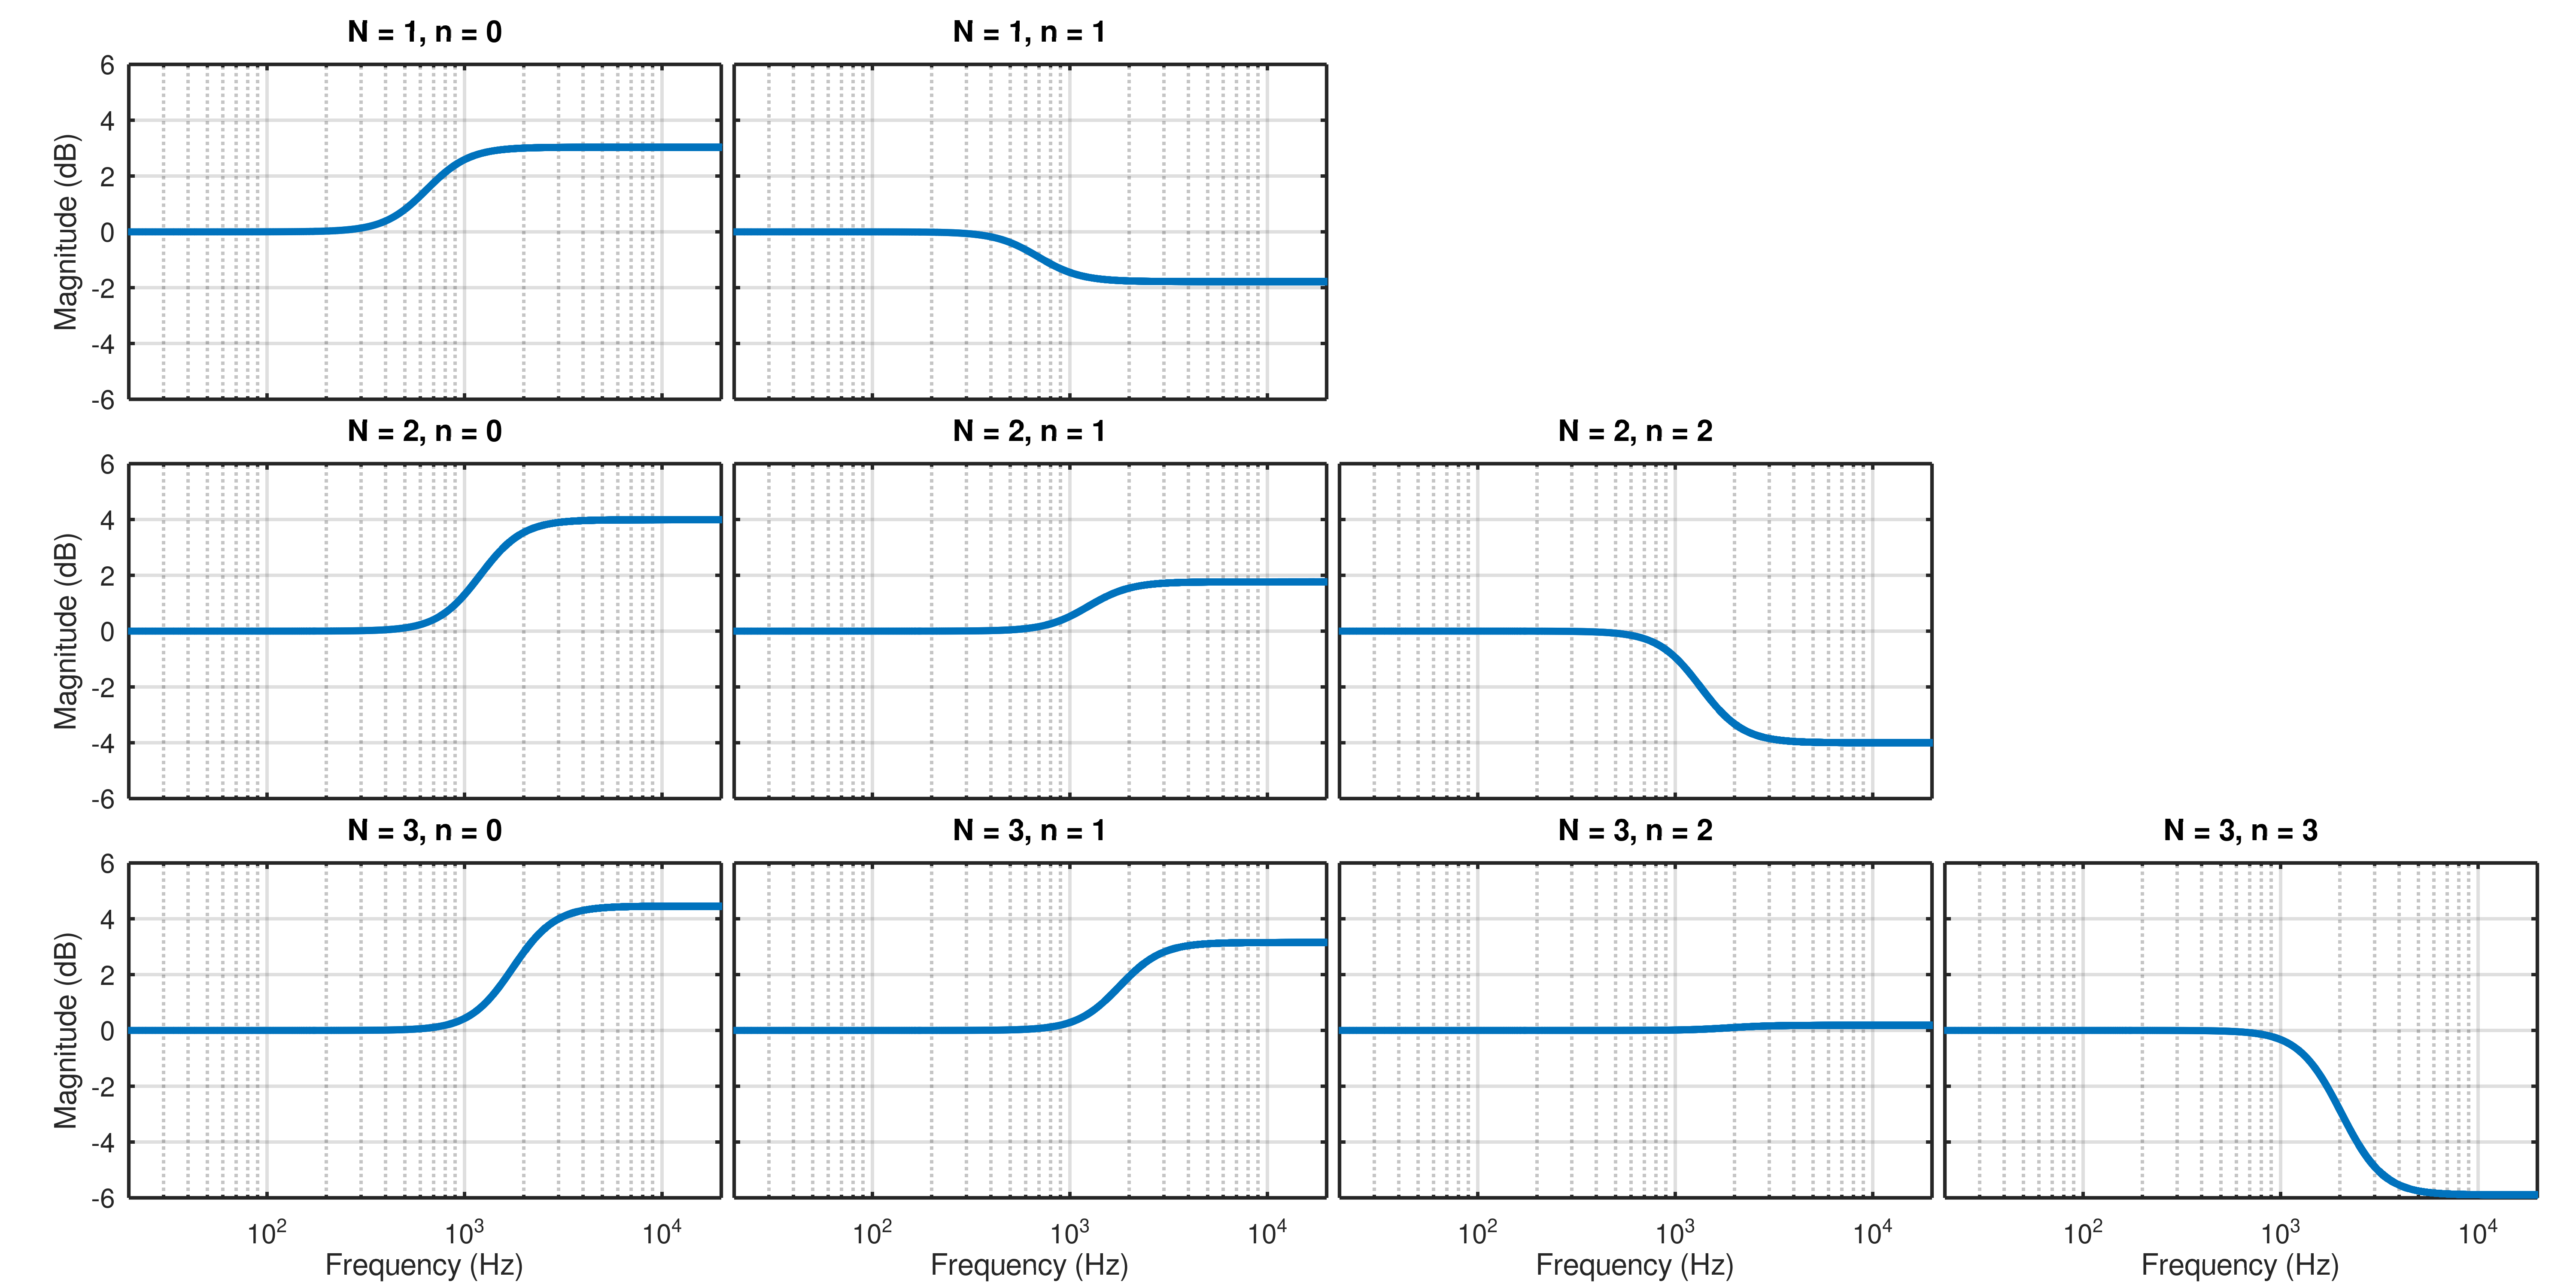
\includegraphics[width = \textwidth]{figures/shelf_filters.png}
    \caption{The magnitudes of the psychoacoustic optimisation filters each group of channel for first- to third-order. The $n = 0$ filter is applied to the first ambisonic channel, $n = 1$ to the three first-order order channels, etc.}
    \label{fig:shelf_filters}
\end{figure}

Psychoacoustic optimisation is implemented in \code{AmbisonicOptimFilters}.
In order to apply the optimisation gains in a frequency-dependent manner $\textbf{b}_{N}$ is filtered by shelf filters with a transition frequency set to the limit frequency, unity gain below and $a_{n}$ gain above.

The filters must be phase-matched to ensure correct decoding.
\code{AmbisonicOptimFilters} uses 4th-order Linkwitz-Riley filters for this purpose.
These are implemented as IIR filters, meaning that the optimisation filtering will have low latency suitable for real-time applications.
Linkwitz-Riley filters have the advantageous property that when a low-passed and high-passed signal are summed the magnitude response is flat.
In practice, \code{AmbisonicOptimFilters} applies a low- and high-pass filter to the input, multiplies the low-passed signal by $a_{n}$ and sums it with the high-passed signal.

The magnitude responses of each of the optimisation filters is shown in the \cref{fig:shelf_filters} for orders 1 to 3.

\textbf{Note}: \code{AmbisonicDecoder} and \code{AmbisonicAllRAD} already use \code{AmbisonicOptimFilters} internally. Therefore, psychoacoustic optimisation should not be applied before using these decoders.

\subsection{\code{AmbisonicOptimFilters}}

\subsubsection{Configuration}

Before calling any other functions the object must first be configured by calling \code{Configure()} with the appropriate values. If the values are supported then it will return \code{true} and the object can now be used.

The configuration parameters are:
\begin{itemize}
    \item \textbf{nOrder}: The ambisonic order from 1 to 3.
    \item \textbf{b3D}: A bool to indicate if the signal is to be filtered is 2D (azimuth only) or 3D (azimuth and elevation).
    \item \textbf{nBlockSize}: The maximum number of samples the object is expected to process at a time.
    \item \textbf{sampleRate}: The sample rate of the audio being used e.g. 44100 Hz, 48000 Hz etc. This must be an integer value greater than zero.
\end{itemize}

\subsubsection{Set Custom Optimisation Gains}

\code{AmbisonicOptimFilters} defaults to using max $r_{E}$ optimisation. However, the user can supply their own optimisation gains to be applied to the high frequency shelf using \code{SetHighFrequencyGains()}. The number of gains should be equal to $N + 1$.

\subsubsection{Apply Optimisation Filters}

A B-format signal can be optimised using the \code{Process()} function. The input signal is replaced by the optimised signal.

The inputs are:
\begin{itemize}
    \item \textbf{pBFSrcDst}: A pointer to the source B-format signal that is replaced with the processed signal.
    \item \textbf{nSamples}: The length of the input signal in samples.
\end{itemize}

\subsection{Code Example}
\begin{lstlisting}[language=C++]
#include "Ambisonics.h"

using namespace spaudio;

const unsigned int sampleRate = 48000;
const int nBlockLength = 512;

// Higher ambisonic order means higher spatial resolution and more channels required
const unsigned int nOrder = 1;
// Set the fade time to the length of one block
const float fadeTimeInMilliSec = 1000.f * (float)nBlockLength / (float)sampleRate;

std::vector<float> sinewave(nBlockLength);
// Fill the vector with a sine wave
for (int i = 0; i < nBlockLength; ++i)
    sinewave[i] = (float)std::sin((float)M_PI * 2.f * 440.f * (float)i / (float)sampleRate);

// B-format buffer
BFormat myBFormat;
myBFormat.Configure(nOrder, true, nBlockLength);
myBFormat.Reset();

// Encode the signal to Ambisonics
AmbisonicEncoder myEncoder;
myEncoder.Configure(nOrder, true, sampleRate, 0);
PolarPosition<float> position;
position.azimuth = 0;
position.elevation = 0;
position.distance = 1.f;
myEncoder.SetPosition(position);
myEncoder.Reset();
myEncoder.Process(sinewave.data(), nBlockLength, &myBFormat);

// Set up the optimisation filters
AmbisonicOptimFilters myOptim;
myOptim.Configure(nOrder, true, nBlockLength, sampleRate);

// Filter the Ambisonics signal
myOptim.Process(&myBFormat, nBlockLength);
\end{lstlisting}

\section{Ambisonic Decoding}\label{AmbiDecoding}

\subsection{Theory and Implementation Details}
An ambisonic signal cannot be played back directly.
A decoder is required to convert the signal from the spherical harmonic representation to either loudspeaker signals (implemented in \code{AmbisonicDecoder} and \code{AmbisonicAllRAD}) or headphone signals (implemented in \code{AmbisonicBinauralizer}).

An ambisonic signal of order $N$ can be decoded to a set of loudspeakers using a decoding matrix $\textbf{D}_{N}^{\mathrm{SN3D}}$ which has size $M \times (N+1)^2$ where $M$ is the total number of loudspeakers. The output loudspeaker signal $\textbf{x}(t)$ is given by

\begin{equation}\label{eqn:decode}
\textbf{x}(t) = \textbf{D}_{N}^{\mathrm{SN3D}} \textbf{b}_{N}(t).
\end{equation}

The decoding matrix can be calculated using a number of different methods \cite{Zotter2012, Zotter2012a, Poletti2005}. If the loudspeaker layout is regularly distributed on a sphere then decoding can be performed simply by sampling the ambisonic signal at each of the directions of the loudspeakers, known as a sampling ambisonic decoder (SAD) \cite{Zotter2019}.
The sampling decoding matrix $\textbf{D}_{N}$ is
\begin{equation}
    \textbf{D}_{N}^{\mathrm{SN3D}} = \frac{1}{\sqrt{M}} \left[ \tilde{\textbf{y}}_{N}(\theta_{1}, \phi_{1}), \tilde{\textbf{y}}_{N}(\theta_{2}, \phi_{2}), \ldots, \tilde{\textbf{y}}_{N}(\theta_{M}, \phi_{M}) \right]^{\mathrm{T}}\mathrm{diag}(\textbf{q}_{N}) = \frac{1}{\sqrt{M}} \tilde{\textbf{Y}}_{N}^{\mathrm{T}}\mathrm{diag}(\textbf{q}_{N})
\end{equation}
where $\tilde{\textbf{y}}_{\texttt{N}}(\theta_{m}, \phi_{m})$ is the vector of spherical harmonics of the $m$-th loudspeaker direction \textbf{with N3D normalisation} and $\textbf{q}_{\texttt{N}}$ is a vector of gains to convert $\textbf{b}_{N}(t)$ from SN3D to N3D normalisation.

\subsubsection{Decoding to Irregular Loudspeaker Layouts Using Non-Linear Optimisation}\label{AmbiIrregularDecoder}

\begin{figure}[tbp]
  \centering

  \begin{subfigure}{0.32\textwidth}
    \includegraphics[width=\linewidth]{figures/ldspkGains_5p0_o1.png}
    \caption{\centering First-order 5.1 gains}
  \end{subfigure}
  \hfill
  \begin{subfigure}{0.32\textwidth}
    \includegraphics[width=\linewidth]{figures/ldspkGains_5p0_o2.png}
    \caption{\centering Second-order 5.1 gains}
  \end{subfigure}
  \hfill
    \begin{subfigure}{0.32\textwidth}
    \includegraphics[width=\linewidth]{figures/ldspkGains_5p0_o3.png}
    \caption{\centering Third-order 5.1 gains}
  \end{subfigure}
  \newline
  \begin{subfigure}{0.32\textwidth}
    \includegraphics[width=\linewidth]{figures/ldspkGains_7p0_o1.png}
    \caption{\centering First-order 7.1 gains}
  \end{subfigure}
  \hfill
    \begin{subfigure}{0.32\textwidth}
    \includegraphics[width=\linewidth]{figures/ldspkGains_7p0_o2.png}
    \caption{\centering Second-order 7.1 gains}
  \end{subfigure}
  \hfill
  \begin{subfigure}{0.32\textwidth}
    \includegraphics[width=\linewidth]{figures/ldspkGains_7p0_o3.png}
    \caption{\centering Third-order 7.1 gains}
  \end{subfigure}
  \hfill
  \caption{Loudspeaker gains for 5.1 and 7.1 arrays for first- to third-order Ambisonics. The directions of the loudspeakers are shown as red circles.}
  \label{fig:irregular_loudspeaker_gains}
\end{figure}

If the layout is irregular, such as the ITU 5.1 and 7.1 layouts, then finding a suitable decoding method becomes more complex.
A significant limitation is that most decoder calculation methods require at least as many loudspeakers as there are ambisonic channels.
This limits 5.1 to first-order.
Wiggins \cite{Wiggins2007} used an optimisation technique that uses the Gerzon velocity and energy vectors \cite{Gerzon1992a}, along with the total pressure and energy sum of the loudspeaker gains, to calculate an optimised decoder for the 5.1 layout.
Due to the optimisation method the higher order spherical harmonics are able to contribute, meaning decoders can be obtained for first- to third-order.

The 5.1 decoders in \libspataud were kindly provided by Bruce Wiggins. 
The decoders for the 7.1 layout were generated using a method inspired by the non-linear optimisation work of Wiggins.
A decoder derived in the manner should not have psychoacoustic optimisation gains or filters (see \cref{AmbiShelves}) applied since the desired optimisations were factored into the decoder optimisation.

Figure \ref{fig:irregular_loudspeaker_gains} shows the gains of each of the loudspeakers for the 5.1 and 7.1 arrays for the orders 1 to 3 with the decoders in \libspataud.
The use of higher-order harmonics is particularly evident in the asymmetric shape of the two rear-surround speakers of the 5.1 layout for third-order.

Figure \ref{fig:irregular_loudspeaker_levels} shows the mean level of the decoders for sources around the horizontal.
It shows that there is in a small level variation with source position around the horizontal at most 3.5 dB for the third-order 5.1 decoder.
Consistent level across source directions is important in maintaining the balance of the sound scene when several sources have been panned to different directions.

\begin{figure}[tbp]
  \centering
  \begin{subfigure}{0.45\textwidth}
    \includegraphics[width=\linewidth]{figures/gainSums_5p0.png}
    \caption{\centering 5.1 array}
  \end{subfigure}
  \hfill
  \begin{subfigure}{0.45\textwidth}
    \includegraphics[width=\linewidth]{figures/gainSums_7p0.png}
    \caption{\centering 7.1 array}
  \end{subfigure}
    \caption{The sum of the loudspeaker gains for 5.1 and 7.1 arrays for source positions on the horizontal.
    The first-order levels are shown in blue, second-order in red, and third-order in yellow.
    The loudspeaker directions are shown as red circles.}
  \label{fig:irregular_loudspeaker_levels}
\end{figure}

\subsubsection{Decoding to Irregular Loudspeaker Layouts Using AllRAD}

The AllRAD method \cite{Zotter2012a} first decodes the signal to a spherically regular t-design virtual loudspeaker layout and then uses VBAP \cite{Pulkki1997} to pan the virtual loudspeakers to the real layout.
The aim is to allow for optimal decoding to the virtual loudspeaker layout and then to spatialise this with a robust panning algorithm.

Additional imaginary loudspeakers can also be included in the main real loudspeaker layout to help when decoding to, for example, a dome.

The AllRAD method is the preferred decoding method of the EBU Audio Definition Model renderer (Recommendation ITU-R BS.2127-1) and Alliance For Open Media's Immersive Audio Model and Formats (IAMF) specification (\href{https://aomediacodec.github.io/iamf/}{https://aomediacodec.github.io/iamf/}).

\subsection{\code{AmbisonicDecoder}}\label{AmbisonicDecoder}

\code{AmbisonicDecoder} decodes an Ambisonics signal to either predefined or custom layouts using one of several methods:

\begin{itemize}
    \item the SAD method: sampling at each of the specified loudspeaker directions. This is suboptimal for any layout that is not regular on the sphere.
    \item optimised decoder: the 5.1 and 7.1 preset layouts use the non-linearly optimised decoder matrices described above, since the SAD method is particularly unsuited to these layouts. The preset decoder matrices are loaded automatically if either of those layouts are selected or if a custom array that matches the directions is defined.
    \item user decoder definition: the user can define the decoder matrix coefficients directly for the specified layout. This means the class can be used with any decoding method that the user requires. See \href{#cambisonicdecoder-set-custom-decoder-coefficients}{here} for more details on how to set a custom decoder matrix.
\end{itemize}

When a decoder matrix other than one of the presets is used \code{AmbisonicDecoder} applies shelf filtering to psychoacoustically optimise the decoded signal. Read more about psychoacoustic optimisation \href{AmbisonicOptimisation.md}{here}.

\subsubsection{Configuration}

Before calling any other functions the object must first be configured by calling \code{Configure()} with the appropriate values. If the values are supported then it will return \code{true} and the object can now be used.

The configuration parameters are:
\begin{itemize}
    \item \textbf{nOrder}: The ambisonic order from 1 to 3.
    \item \textbf{b3D}: A bool to indicate if the signal to be decoded is 2D (azimuth only) or 3D (azimuth and elevation).
    \item \textbf{nBlockSize}: The maximum number of samples the decoder is expected to process at a time.
    \item \textbf{sampleRate}: The sample rate of the audio being used e.g. 44100 Hz, 48000 Hz etc. This must be an integer value greater than zero.
    \item \textbf{nSpeakerSetup}: Choice of loudspeaker layout from one of the predefined options or to indicate use of a custom layout. Note that the 5.1 and 7.1 layouts \textbf{do not} use the ITU ordering. They use L/R/Ls/Rs/C/LFE and L/R/Ls/Rs/Lr/Rr/C/LFE respectively. This matches the channel ordering in VLC media player.
    \item \textbf{nSpeakers}: The total number of loudspeakers if a custom layout is used. This is ignored if one of the predefined layouts is selected.
\end{itemize}

\subsubsection{Set Custom Decoder Coefficients}

The \code{SetCoefficient()} function can be used to define a custom decoder for the currently selected layout.

The parameters are:
\begin{itemize}
    \item \textbf{nSpeaker}: The index of the loudspeaker for which the coefficient is to be set.
    \item \textbf{nChannel}: The index of the corresponding Ambisonic channel for which the coefficient is to be set.
    \item \textbf{fCoeff}: The decoder matrix coefficient.
\end{itemize}

The following code will set the decoder matrix to hold the values stored in \code{myDecMat}.

\begin{lstlisting}[language=C++]
for (int iSpeaker = 0; iSpeaker < nLdspk; ++iSpeaker)
    for (int iCoeff = 0; iCoeff < nAmbiComponents; ++iCoeff)
    {
        myDecoder.SetCoefficients(iSpeaker, iCoeff, myDecMat[iSpeaker][iCoeff]);
    }
\end{lstlisting}

\textbf{Note}: Calling \code{Refresh()} will overwrite any coefficients set in this way and replace them with the default values for the selected layout (either a SAD matrix or a preset).

\subsubsection{Decoding a Signal}

A B-format signal can be decoded to the loudspeaker signals using the \code{Process()} function. The processing is non-replacing, so the original B-format signal is unchanged and the decoded signal is contained in the output array.

The inputs are:
\begin{itemize}
    \item \textbf{pBFSrc}: A pointer to the source B-format signal.
    \item \textbf{nSamples}: The length of the input signal in samples.
    \item \textbf{ppDst}: Array of pointers of size nLdspk x nSamples containing the decoded signal.
\end{itemize}

\subsection{\code{AmbisonicDecoder} Code Example}

This example shows how to decode an Ambisonics signal to a 5.1 loudspeaker layout. It loads the optimised preset decoder for this layout automatically.

\begin{lstlisting}[language=C++]
#include "Ambisonics.h"

using namespace spaudio;

const unsigned int sampleRate = 48000;
const int nBlockLength = 512;

// Higher ambisonic order means higher spatial resolution and more channels required
const unsigned int nOrder = 1;

std::vector<float> sinewave(nBlockLength);
// Fill the vector with a sine wave
for (int i = 0; i < nBlockLength; ++i)
    sinewave[i] = (float)std::sin((float)M_PI * 2.f * 440.f * (float)i / (float)sampleRate);

// B-format buffer
BFormat myBFormat;
myBFormat.Configure(nOrder, true, nBlockLength);
myBFormat.Reset();

// Encode the signal to Ambisonics
AmbisonicEncoder myEncoder;
myEncoder.Configure(nOrder, true, sampleRate, 0);
PolarPosition<float> position;
position.azimuth = 0;
position.elevation = 0;
position.distance = 1.f;
myEncoder.SetPosition(position);
myEncoder.Reset();
myEncoder.Process(sinewave.data(), nBlockLength, &myBFormat);

// Set up the decoder for a 5.1 layout
AmbisonicDecoder myDecoder;
myDecoder.Configure(nOrder, true, nBlockLength, sampleRate, Amblib_SpeakerSetUps::kAmblib_51);

// Configure buffers to hold the decoded signal
const unsigned int nLdspk = myDecoder.GetSpeakerCount();
float** ldspkOut = new float* [nLdspk];
for (int iLdspk = 0; iLdspk < nLdspk; ++iLdspk)
    ldspkOut[iLdspk] = new float[nBlockLength];

// Decode the Ambisonics signal
myDecoder.Process(&myBFormat, nBlockLength, ldspkOut);

// Cleanup
for (unsigned iLdspk = 0; iLdspk < nLdspk; ++iLdspk)
    delete[] ldspkOut[iLdspk];
delete[] ldspkOut;
\end{lstlisting}

\subsection{\code{AmbisonicAllRAD}}\label{AmbisonicAllRAD}

\code{AmbisonicAllRAD} decodes an Ambisonics signal to a layout defined in the ADM renderer specification (Recommendation ITU-R BS.2127-1) and AOM's IAMF specification (\href{https://aomediacodec.github.io/iamf/}{https://aomediacodec.github.io/iamf/}). It does not currently support decoding to arbitrary loudspeaker layouts.

\code{AmbisonicAllRAD} optionally applies shelf filtering to psychoacoustically optimise the decoded signal. Read more about psychoacoustic optimisation \href{AmbisonicOptimisation.md}{here}.

\subsubsection{Configuration}

Before calling any other functions the object must first be configured by calling \code{Configure()} with the appropriate values. If the values are supported then it will return \code{true} and the object can now be used.

The configuration parameters are:
\begin{itemize}
    \item \textbf{nOrder}: The ambisonic order from 1 to 3.
    \item \textbf{nBlockSize}: The maximum number of samples the decoder is expected to process at a time.
    \item \textbf{sampleRate}: The sample rate of the audio being used e.g. 44100 Hz, 48000 Hz etc. This must be an integer value greater than zero.
    \item \textbf{layoutName}: The name of the loudspeaker layout. This must be one of those specified in the ADM or IAMF specifications. The valid names are:
    \begin{itemize}
        \item \code{"0+2+0"}: BS.2051-3 System A (Stereo)
        \item \code{"0+4+0"}: Quad
        \item \code{"0+5+0"}: BS.2051-3 System B (5.1)
        \item \code{"2+5+0"}: BS.2051-3 System C (5.1.2)
        \item \code{"4+5+0"}: BS.2051-3 System D (5.1.4)
        \item \code{"4+5+1"}: BS.2051-3 System E
        \item \code{"3+7+0"}: BS.2051-3 System F
        \item \code{"4+9+0"}: BS.2051-3 System G
        \item \code{"9+10+3"}: BS.2051-3 System H
        \item \code{"0+7+0"}: BS.2051-3 System I (7.1)
        \item \code{"4+7+0"}: BS.2051-3 System J (7.1.4)
        \item \code{"2+7+0"}: 7.1.2 (IAMF v1.0.0-errata)
        \item \code{"2+3+0"}: 3.1.2 (IAMF v1.0.0-errata)
        \item \code{"9+10+5"}: EBU Tech 3369 (BEAR) 9+10+5 - 9+10+3 with LFE1 \& LFE2 removed and B+135 \& B-135 added
    \end{itemize}
    \item \textbf{useLFE}: If \code{true} then the decoded signal will include the LFE channels. If \code{false} then the LFE channels will be excluded i.e. a 0+5+0 (5.1) signal will be output as a 5-channel signal instead of a 6-channel one.
    \item \textbf{useOptimFilts}: (Optional) \code{false} by default. If true, then \href{AmbisonicOptimsiation.md}{psychoacoustic optimisation filters} will be applied before decoding the signal.
\end{itemize}

\subsubsection{Decoding a Signal}

A B-format signal can be decoded to the loudspeaker signals using the \code{Process()} function. The processing is non-replacing, so the original B-format signal is unchanged, and the decoded signal is contained in the output array.

The inputs are:
\begin{itemize}
    \item \textbf{pBFSrc}: A pointer to the source B-format signal.
    \item \textbf{nSamples}: The length of the input signal in samples.
    \item \textbf{ppDst}: Array of pointers of size nLdspk x nSamples containing the decoded signal.
\end{itemize}

\subsection{\code{AmbisonicAllRAD} Code Example}

This example shows how to decode an Ambisonics signal to an ITU 5.1 loudspeaker layout using the AllRAD method.

\begin{lstlisting}[language=C++]
#include "Ambisonics.h"

using namespace spaudio;

const unsigned int sampleRate = 48000;
const int nBlockLength = 512;

// Higher ambisonic order means higher spatial resolution and more channels required
const unsigned int nOrder = 1;

std::vector<float> sinewave(nBlockLength);
// Fill the vector with a sine wave
for (int i = 0; i < nBlockLength; ++i)
    sinewave[i] = (float)std::sin((float)M_PI * 2.f * 440.f * (float)i / (float)sampleRate);

// B-format buffer
BFormat myBFormat;
myBFormat.Configure(nOrder, true, nBlockLength);
myBFormat.Reset();

// Encode the signal to Ambisonics
AmbisonicEncoder myEncoder;
myEncoder.Configure(nOrder, true, sampleRate, 0);
PolarPosition<float> position;
position.azimuth = 0;
position.elevation = 0;
position.distance = 1.f;
myEncoder.SetPosition(position);
myEncoder.Reset();
myEncoder.Process(sinewave.data(), nBlockLength, &myBFormat);

// Set up the decoder for a 5.1 layout
AmbisonicAllRAD myDecoder;
myDecoder.Configure(nOrder, nBlockLength, sampleRate, "0+5+0");

// Configure buffers to hold the decoded signal
const unsigned int nLdspk = myDecoder.GetSpeakerCount();
float** ldspkOut = new float* [nLdspk];
for (int iLdspk = 0; iLdspk < nLdspk; ++iLdspk)
    ldspkOut[iLdspk] = new float[nBlockLength];

// Decode the Ambisonics signal
myDecoder.Process(&myBFormat, nBlockLength, ldspkOut);

// Cleanup
for (unsigned iLdspk = 0; iLdspk < nLdspk; ++iLdspk)
    delete[] ldspkOut[iLdspk];
delete[] ldspkOut;
\end{lstlisting}


\section{Ambisonic-to-Binaural Decoding}\label{AmbiToBin}

\subsection{Theory and Implementation Details}
There are several methods for decoding from Ambisonics to binaural \cite{Noisternig2003,schorkhuber2018binaural,Zaunschirm2018}.
In general, decoding is performed by convolution of the ambisonic signal with a matrix of filters.
\texttt{AmbisonicBinauralizer} uses a virtual-speaker approach \cite{Noisternig2003}.

The virtual loudspeaker approach essentially decodes the signal to known loudspeaker array and then applies an HRTF to each of the loudspeakers, which are summed for 2-channel output.
This requires $2\times M$ convolutions, where $M$ is the number of virtual loudspeakers.

In order to reduce the number of convolutions the HRTF of each virtual speaker is scaled by the corresponding ambisonic gains and summed to create a filter for each spherical harmonic. For an HRIR of length $k$ this is calculated using
\begin{equation}
    \mathbf{Z}_{N,ear}^{\mathrm{bin}} = \frac{1}{\sqrt{M}} \left[ \tilde{\textbf{y}}_{N}(\theta_{1}, \phi_{1}), \tilde{\textbf{y}}_{N}(\theta_{2}, \phi_{2}), \ldots, \tilde{\textbf{y}}_{N}(\theta_{M}, \phi_{M}) \right] \mathbf{H}_{\mathrm{ear}}
\end{equation}
where $\mathbf{Z}_{N,ear}^{\mathrm{bin}}$ is a matrix of 
size $(N+1)^{2} \times k$ containing the spherical harmonic decomposition of the loudspeaker array HRIRs, $\mathbf{H}_{\mathrm{ear}}$ is an $M\times k$ matrix containing the HRIRs corresponding to each of the loudspeaker directions for the left or right ear.
This leads to $2\times (N + 1)^2$ convolutions which can be calculated using
\begin{equation}\label{eq:binaural_output}
    x_{\mathrm{bin}}^{ear}(t) = \sum_{i = 0}^{(N+1)^{2}} q_{i} z_{i}^{ear}(t) \circledast b_{i}(t)
\end{equation}
where $z_{i}^{ear}(t)$ is the filter in the $i$-th row of $\mathbf{Z}_{\mathrm{N,ear}}^{\mathrm{bin}}$, $b_{i}(t)$ is the $i$-th term in the ambisonic signal $\textbf{b}_{N}(t)$, and $q_{i}$ is the $i$-th element of $\mathbf{q}_{N}$ which contains gains that convert the input signal from SN3D to N3D.

The number of convolutions can be reduced further to only $(N+1)^2$ convolutions if the head is assumed to be symmetric \cite{politis2016jsambisonics}.
This is done by calculating the convolutions in \cref{eq:binaural_output} for one ear and storing them.
They are summed for the first ear directly.
For the opposite ear the spherical harmonics that are left-right symmtertic have their polarity inverted and before being summed.

\subsubsection{Virtual Loudspeaker Layout Choices}

\begin{figure}[tbp]
  \centering

  \begin{subfigure}{0.3\textwidth}
    \includegraphics[width=\linewidth]{figures/A_dodeca.png}
    \caption{\centering Total amplitude}
  \end{subfigure}
  \hfill
  \begin{subfigure}{0.3\textwidth}
    \includegraphics[width=\linewidth]{figures/errAzV_dodeca.png}
    \caption{\centering Velocity vector error}
  \end{subfigure}
  \hfill
    \begin{subfigure}{0.3\textwidth}
    \includegraphics[width=\linewidth]{figures/rV_dodeca.png}
    \caption{\centering Velocity vector mag.}
  \end{subfigure}
  \newline
    \begin{subfigure}{0.3\textwidth}
    \includegraphics[width=\linewidth]{figures/E_dodeca.png}
    \caption{\centering Total energy}
  \end{subfigure}
  \hfill
    \begin{subfigure}{0.3\textwidth}
    \includegraphics[width=\linewidth]{figures/errAzE_dodeca.png}
    \caption{\centering Energy vector error}
  \end{subfigure}
  \hfill
  \begin{subfigure}{0.3\textwidth}
    \includegraphics[width=\linewidth]{figures/rE_dodeca.png}
    \caption{\centering Energy vector mag.}
  \end{subfigure}
    \caption{The quality measures for a basic decoder (top row) and max $r_{\mathrm{E}}$ decoder (bottom row) as a function of the source direction across the whole sphere for a third-order decoding to a dodecahedral loudspeaker array.
    The directions of the loudspeakers are shown as red circles.}
  \label{fig:dodeca_third_order}
\end{figure}

For first-order signals \code{AmbisonicBinauralizer} uses a virtual layout on the vertices of a cube (8 virtual loudspeakers).
For second- and third-order a virtual layout on the vertices of a dodecahedron (20 virtual loudspeakers) is used.
Therefore, in both cases, preprocessing the HRTFs reduces the number of convolutions required (from 8 to 4 for first-order and 20 to 9 or 16 for second- and third-order respectively).
This meets a requirement of \libspataud to minimise its CPU use.

A cube was chosen for first-order because it is a mathematically ideal layout for this order.
The dodocahedron was chosen because it provides good results for second- and third-order order and 8 of its 20 loudspeaker directions coincide directly with the cube layout.
This allows for the number of HRTFs stored for both layouts to be only 20, meeting a requirement that \libspataud be lightweight.

Figure \ref{fig:dodeca_third_order} shows the total loudspeaker gain and energy for the dodecahedron for third-order (first- and second-order are now shown because they have equal performance for all source directions).
It also shows the difference between the panning direction and velocity and energy vectors \cite{Gerzon1992a}, representing a prediction of perceived direction for low and high frequencies respectively.
Finally, it also shows the velocity and energy vector magnitudes, for which a value of 1 is ideal (although an energy vector magnitude of 1 is not possible for a sound source reproduced by more than one loudspeaker).

The figure shows that both amplitude and energy are constant for all source directions.
The velocity vector has perfect localisation and magnitude, indicating that at low frequencies the decoder is also performing ideally.
The max $r_{\mathrm{E}}$ decoder for high frequencies shows small deviations between the source direction and the energy vector prediction.
However, the maximum error is only 6.5\deg.
The energy vector magnitude also exhibits some variation with source position.
This may result in small variations in the perceived source width, but this effect will be small.

\subsubsection{Psychoacoustic Optimisation}

As outlined in \cref{AmbiShelves} shelf filtering can be applied to Ambisonics signal so that they are decoded in a psychoacoustically optimised manner.

\subsection{\code{AmbisonicBinauralizer}}

\subsubsection{Configuration}

Before calling any other functions the object must first be configured by calling \code{Configure()} with the appropriate values. If the values are supported then it will return \code{true} and the object can now be used.

The configuration parameters are:
\begin{itemize}
    \item \textbf{nOrder}: The ambisonic order from 1 to 3.
    \item \textbf{b3D}: A bool to indicate if the signal is to be decoded is 2D (azimuth only) or 3D (azimuth and elevation).
    \item \textbf{nBlockSize}: The maximum number of samples the decoder is expected to process at a time.
    \item \textbf{sampleRate}: The sample rate of the audio being used e.g. 44100 Hz, 48000 Hz etc. This must be an integer value greater than zero.
    \item \textbf{tailLength}: The value is replaced with the length of the HRIRs used for the binauralisation.
    \item \textbf{HRTFPath}: An optional path to the .SOFA file containing the HRTF. If no path is supplied and the \code{HAVE\_MIT\_HRTF} compiler flag is used, then the MIT HRTF will be used.
    \item \textbf{lowCpuMode}: (Optional) If this is set to true (its default value), then the symmetric head assumption is used to reduce CPU usage \cite{politis2016jsambisonics}.
\end{itemize}

\subsubsection{Decoding a Signal}

A B-format signal can be decoded to the binaural signals using the \code{Process()} function. The processing is non-replacing, so the original B-format signal is unchanged, and the decoded signal is contained in the output array.

The inputs are:
\begin{itemize}
    \item \textbf{pBFSrc}: A pointer to the source B-format signal.
    \item \textbf{ppDst}: Array of pointers of size 2 x nSamples containing the binaurally decoded signal.
    \item \textbf{nSamples}: (Optional) The length of the input signal in samples. If this is not supplied, then \code{nBlockSize} samples are assumed.
\end{itemize}

\subsection{Code Example}

This example shows how to decode an Ambisonics signal to binaural.

\begin{lstlisting}[language=C++]
#include "Ambisonics.h"

using namespace spaudio;

const unsigned int sampleRate = 48000;
const int nBlockLength = 512;

// Higher ambisonic order means higher spatial resolution and more channels required
const unsigned int nOrder = 1;

std::vector<float> sinewave(nBlockLength);
// Fill the vector with a sine wave
for (int i = 0; i < nBlockLength; ++i)
    sinewave[i] = (float)std::sin((float)M_PI * 2.f * 440.f * (float)i / (float)sampleRate);

// B-format buffer
BFormat myBFormat;
myBFormat.Configure(nOrder, true, nBlockLength);
myBFormat.Reset();

// Encode the signal to Ambisonics
AmbisonicEncoder myEncoder;
myEncoder.Configure(nOrder, true, sampleRate, 0);
PolarPosition<float> position;
position.azimuth = (float)M_PI * 0.5f;
position.elevation = 0;
position.distance = 1.f;
myEncoder.SetPosition(position);
myEncoder.Reset();
myEncoder.Process(sinewave.data(), nBlockLength, &myBFormat);

// Set up the binaural decoder
AmbisonicBinauralizer myDecoder;
unsigned int tailLength = 0;
myDecoder.Configure(nOrder, true, sampleRate, nBlockLength, tailLength);

// Configure buffers to hold the decoded signal
const unsigned int nEar = 2;
float** earOut = new float* [nEar];
for (int iEar = 0; iEar < nEar; ++iEar)
    earOut[iEar] = new float[nBlockLength];

// Decode the Ambisonics signal
myDecoder.Process(&myBFormat, earOut, nBlockLength);

// Cleanup
for (unsigned iEar = 0; iEar < nEar; ++iEar)
    delete[] earOut[iEar];
delete[] earOut;
\end{lstlisting}

\chapter{Speaker Binauralization}\label{Binauralization}

\section{Theory and Implementation Details}
Binauralization of a loudspeaker array uses a simple method.
First, a pair of head-related impulse responses (HRIRs) for each of the loudspeaker directions is convolved with the signal of that loudspeaker.
The convolved signals are summed to give a final 2-channel binaural signal for listening over headphones.
\begin{equation}
    z_{ear}(t) = \sum_{m = 0}^{M - 1} h_{m,ear}(t)\circledast x_{m}(t)
\end{equation}
where $z_{ear}(t)$ is the signal at the left or right ear, $h_{ear}$ is the corresponding HRIR for the left/right ear, $x_{m}(t)$ is the signal of the $m$-th loudspeaker and $M$ is the total number of loudspeakers.

\code{SpeakersBinauralizer} provides a simple convolution of a set of supplied loudspeaker signals with a pair of HRTFs (one for each ear).
The convolution is implemented in the frequency domain using an overlap-add algorithm.

If \code{libmysofa} is activated at compile time then the HRTF can be loaded from a .SOFA file, allowing for the use of custom HRTFs.
Custom HRTFs allow for users to potentially load their own HRTF, giving highly personalised rendering.

\section{\code{SpeakersBinauralizer}}

\subsection{Configuration}

Before calling any other functions the object must first be configured by calling \code{Configure()} with the appropriate values. If the values are supported then it will return \code{true} and the object can now be used.

The configuration parameters are:
\begin{itemize}
    \item \textbf{sampleRate}: The sample rate of the audio being used e.g. 44100 Hz, 48000 Hz etc. This must be an integer value greater than zero.
    \item \textbf{nBlockSize}: The maximum number of samples the decoder is expected to process at a time.
    \item \textbf{speakers}: A pointer to an array of \code{AmbisonicSpeaker} holding the speaker directions.
    \item \textbf{nSpeakers}: The number of speakers to be binauralized.
    \item \textbf{tailLength}: The value is replaced with the length of the HRIRs used for the binauralisation.
    \item \textbf{HRTFPath}: An optional path to the .SOFA file containing the HRTF. If no path is supplied and the \code{HAVE\_MIT\_HRTF} compiler flag is used, then the MIT HRTF will be used.
\end{itemize}

\subsection{Binauralizing a Signal}

A set of loudspeaker signals can be decoded to the binaural signals using the \code{Process()} function. The processing is non-replacing, so the original loudspeaker signals are unchanged, and the decoded signal is contained in the output array.

The inputs are:
\begin{itemize}
    \item \textbf{pBFSrc}: A pointer to the source B-format signal.
    \item \textbf{ppDst}: Array of pointers of size 2 x nBlockSize containing the binaurally decoded signal.
\end{itemize}

\subsubsection{Code Example}

This example shows how to convert a set of loudspeaker signals to a 2-channel binaural signal.

\begin{lstlisting}[language=C++]
#include "SpeakersBinauralizer.h"

using namespace spaudio;

const unsigned int sampleRate = 48000;
const int nBlockLength = 512;

// Configure the speaker layout
const unsigned int nSpeakers = 5;
AmbisonicSpeaker speakers[nSpeakers];
speakers[0].SetPosition({ 30.f / 180.f * (float)M_PI, 0.f, 1.f }); // L
speakers[1].SetPosition({ -30.f / 180.f * (float)M_PI, 0.f, 1.f }); // R
speakers[2].SetPosition({ 0.f / 180.f * (float)M_PI, 0.f, 1.f }); // C
speakers[3].SetPosition({ 110.f / 180.f * (float)M_PI, 0.f, 1.f }); // Ls
speakers[4].SetPosition({ -110.f / 180.f * (float)M_PI, 0.f, 1.f }); // Rs

// Configure buffers to hold the 5.0 signal
float** ldspkInput = new float* [5];
for (int iLdspk = 0; iLdspk < 5; ++iLdspk)
{
    ldspkInput[iLdspk] = new float[nBlockLength];
    // Fill L and C channels, panning the signal to half way between both speakers
    for (int i = 0; i < nBlockLength; ++i)
        ldspkInput[iLdspk][i] = iLdspk == 0 || iLdspk == 2 ? (float)std::sin((float)M_PI * 2.f * 440.f * (float)i / (float)sampleRate) : 0.f;
}

// Set up the binauralizer
SpeakersBinauralizer myBinaural;
unsigned int tailLength = 0;
myBinaural.Configure(sampleRate, nBlockLength, speakers, nSpeakers, tailLength);

// Configure buffers to hold the decoded signal
const unsigned int nEar = 2;
float** earOut = new float* [nEar];
for (int iEar = 0; iEar < nEar; ++iEar)
    earOut[iEar] = new float[nBlockLength];

// Convert the loudspeaker signals to binaural
myBinaural.Process(&ldspkInput[0], earOut);

// Cleanup
for (unsigned iEar = 0; iEar < nEar; ++iEar)
    delete[] earOut[iEar];
delete[] earOut;
for (unsigned iLdspk = 0; iLdspk < nSpeakers; ++iLdspk)
    delete[] ldspkInput[iLdspk];
delete[] ldspkInput;
\end{lstlisting}

\chapter{Object Spatialisation}\label{ObjectSpatialisation}

\section{Theory and Implementation Details}

Object-based panning is the process of placing a mono signal at an arbitrary position in a loudspeaker layout by distributing its energy across the available loudspeakers.  
\texttt{ObjectPanner} implements Vector Base Amplitude Panning (VBAP) following the algorithm described in the Audio Definition Model (ADM) renderer specification \cite{Pulkki1997, ITU2127}.

\texttt{ObjectPanner} can be used to pan a mono sound source as a point source on a given loudspeaker array.
More advanced Object rendering is possible with the \texttt{Renderer} class that allows for metadata to specify additional parameters, such as object extent.

\subsection{VBAP Algorithm}

Classic VBAP works by selecting a subset of loudspeakers (a base) that encloses the desired source direction and calculating gain factors such that the vector sum of the loudspeaker positions matches the target direction. The gains are normalized to preserve energy.

For a source at direction vector $\mathbf{d}$ and a loudspeaker base matrix $\mathbf{L}$ containing unit vectors in the loudspeaker directions, the gains $\mathbf{g}$ are obtained by solving:

\begin{equation}
\mathbf{L} \mathbf{g} = \mathbf{d}
\end{equation}

with the constraint that all elements of $\mathbf{g}$ are non-negative. The resulting gains $\mathbf{g}'$ are then normalized:

\begin{equation}
\mathbf{g}' = \frac{\mathbf{g}}{\|\mathbf{g}\|}
\end{equation}

\subsection{Gain Interpolation}

To avoid audible artefacts when the source position changes (clicks or ``zipper noise''), \code{ObjectPanner} uses an internal \code{GainInterp} object. When the position is updated, the loudspeaker gain vector is interpolated over a user-specified fade time (typically 10 ms). This ensures smooth transitions.

\section{\code{ObjectPanner}}

The \code{ObjectPanner} class is used to distribute a mono signal across a loudspeaker layout using VBAP. It supports smooth position updates to reduce real-time ``zipper'' effects for moving sources.

\subsection{Configuration}

Before calling any other functions the object must first be configured by calling \code{Configure()} with the appropriate values. If the values are supported then it will return \code{true} and the object can now be used.

The configuration parameters are:

\begin{itemize}
  \item \textbf{layout}: An \code{OutputLayout} to select a supported output layout.
  \item \textbf{sampleRate}: The sample rate of the audio being used (e.g.\ 44100 Hz, 48000 Hz). Must be an integer $> 0$.
  \item \textbf{fadeTimeMilliSec}: The time in milliseconds to fade from an old set of panning gains to another. Lower values reduce latency but may introduce artefacts; higher values increase smoothness at the cost of responsiveness.
\end{itemize}

\subsection{Set Panning Position}

The panning position is set as a polar direction in radians using the \code{SetPosition()} function. It takes a \code{PolarPosition<double>} as input.

\subsection{Panning a Signal}

An array of floats can be panned using either the \code{Process()} or \code{ProcessAccumul()} functions. These two functions process the input signal in the same way. The only difference is that \code{ProcessAccumul()} will add the newly panned signal to the output with an optional gain, whereas \code{Process()} will replace the destination signal with the panned signal.

The inputs are:

\begin{itemize}
  \item \textbf{pfSrc}: A pointer to the mono input signal.
  \item \textbf{nSamples}: The length of the input signal in samples.
  \item \textbf{ppDst}: A pointer to the destination buffer containing one channel per loudspeaker.
  \item \code{nSamplesOut}: The number of samples in the output buffer. Must be at least \code{nSamplesIn + nOffset}.
  \item \code{nOffset}: Optional offset position when writing to the output.
  \item (\texttt{ProcessAccumul()} only) \code{fGain}: Optional gain to apply before accumulation.
\end{itemize}

\subsection{Code Example}

This example shows how to pan a mono sine wave into a 5.1 loudspeaker layout using \texttt{ObjectPanner}.

\begin{lstlisting}[language=C++, basicstyle=\ttfamily\small]
#include "ObjectPanner.h"

using namespace spaudio;

const unsigned int sampleRate = 48000;
const int nBlockLength = 512;

auto layout = OutputLayout::FivePointOne;

ObjectPanner objPanner;
objPanner.Configure(layout, sampleRate, 1000.f * (float)nBlockLength / (float)sampleRate);
unsigned nLdspk = (unsigned)objPanner.GetNumSpeakers();

// Generate a block of sine wave samples
std::vector<float> sinewave(nBlockLength);
for (int i = 0; i < nBlockLength; ++i)
    sinewave[i] = (float)std::sin((float)M_PI * 2.f * 440.f * (float)i / (float)sampleRate);

// Prepare the output stream (5.1 layout)
float** renderStream = new float* [nLdspk];
for (unsigned int i = 0; i < nLdspk; ++i)
{
    renderStream[i] = new float[nBlockLength];
    std::fill(renderStream[i], renderStream[i] + nBlockLength, 0.f);
}

for (float az = 0.f; az < 360.f; az += 1.f)
{
    auto position = PolarPosition<double>{ az, 0.f, 1.f };
    objPanner.SetPosition(position);
    objPanner.Process(sinewave.data(), nBlockLength, renderStream, nBlockLength);
}

for (unsigned iLdspk = 0; iLdspk < nLdspk; ++iLdspk)
    delete[] renderStream[iLdspk];
delete[] renderStream;
\end{lstlisting}

\chapter{Renderer}\label{Renderer}

\section{Overview}

\libspataud includes a renderer for the Audio Definition Model (ADM) renderer detailed in Rec. ITU-R BS.2127-1 \cite{ITU2127}. It also aims to support elements of the AOM's Immersive Audio Model and Formats (IAMF) specification\footnote{\href{https://aomediacodec.github.io/iamf/}{https://aomediacodec.github.io/iamf/}}.

The Renderer specifies rendering methods for Objects, HOA, and DirectSpeaker streams:
\begin{itemize}
    \item Object streams consist of a mono audio signal and metadata which specify how they are spatialised. More details can be read in \cref{AdmObject}.
    \item HOA streams are summed and decoded to the target playback format (loudspeakers or binaural). More details and an example can be found in \cref{AdmHOA}.
    \item DirectSpeaker streams are intended to be sent directly to a specific loudspeaker in the target layout, if it is present.
If it is not present then the DirectSpeaker stream will be spatialised based on the target layout and its associated metadata. More details can be read in \cref{AdmDirectSpeaker}.
\end{itemize}

Rec. ITU-R BS.2127-1 \cite{ITU2127} should be consulted for full details about the rendering algorithms.

\subsubsection{Supported Output Formats}

\code{Renderer} supports all of the loudspeaker layouts specified in \cite{ITU2127} as well as additional ones specified in the IAMF.

The supported ITU layouts are:
\begin{itemize}
    \item \code{"0+2+0"}: BS.2051-3 System A (Stereo)
    \item \code{"0+5+0"}: BS.2051-3 System B (5.1)
    \item \code{"2+5+0"}: BS.2051-3 System C (5.1.2)
    \item \code{"4+5+0"}: BS.2051-3 System D (5.1.4)
    \item \code{"4+5+1"}: BS.2051-3 System E
    \item \code{"3+7+0"}: BS.2051-3 System F
    \item \code{"4+9+0"}: BS.2051-3 System G
    \item \code{"9+10+3"}: BS.2051-3 System H
    \item \code{"0+7+0"}: BS.2051-3 System I (7.1)
    \item \code{"4+7+0"}: BS.2051-3 System J (7.1.4)
\end{itemize}


The additional IAMF layouts are: 
\begin{itemize}
    \item \code{"2+7+0"}: 7.1.2 (IAMF v1.1.0)
    \item \code{"2+3+0"}: 3.1.2 (IAMF v1.1.0)
\end{itemize}

A quad layout is also supported, along with the virtual layout specified in \cite{EBU3369}:
\begin{itemize}
    \item \code{"0+4+0"}: Quad
    \item \code{"9+10+5"}: EBU Tech 3369 (BEAR) 9+10+5 - 9+10+3 with LFE1 and LFE2 removed and B+135 and B-135 added. This is used internally for the binaural rendering.
\end{itemize}

In addition to these loudspeaker layouts, \code{Renderer} implements a custom binaural renderer that is inspired by the BEAR renderer specified in \cite{EBU3369}. Full details on the binaural rendering processing can be read in \cref{AdmBinaural}.

\subsection{\code{Renderer}}

The \code{Renderer} is the only class you will need to interact with to render an a mixture of Object, DirectSpeaker and/or HOA feeds, such as ADM or IAMF. It accepts audio streams and metadata to produce a signal rendered to the specified output format.

Use the class as follows:
\begin{enumerate}
    \item Configure the class by informing it of the different streams it should expect.
    \item Add each stream using the appropriate function i.e. \code{AddHOA()} for an Ambisonics signal.
    \item Once all streams have been added use \code{GetRenderedAudio()}. This clears any internal buffers containing waiting audio.
    \item Repeat steps 2 and 3.
\end{enumerate}

\subsubsection{Configuration}

Before calling any other functions the object must first be configured by calling \code{Configure()} with the appropriate values. If the values are supported then the it will return `true` and the object can now be used.

The configuration parameters are:
\begin{itemize}
    \item \textbf{outputTarget}: The target output layout selected from \code{OutputLayout}.
    \item \textbf{hoaOrder}: The ambisonic order of the signal to be rendered. This also control the order of the HOA processing used for binaural output, so higher should be preferred.
    \item \textbf{nSampleRate}: Sample rate of the streams to be processed.
    \item \textbf{nSamples}: The maximum number of samples in an audio frame to be added to the stream.
    \item \textbf{channelInfo}: Information about the expected stream formats.
    \item \textbf{HRTFPath}: Path to an HRTF SOFA-file to be used when the output layout is binaural.
    \item \textbf{reproductionScreen}: (Optional) Reproduction screen details used for screen scaling/locking.
    \item \textbf{layoutPositions}: (Optional) Real polar positions for each of the loudspeaker in the layout. This is used if they do not exactly match the ITU specification. Note that they must be within the range allowed by the specification.
\end{itemize}

\subsubsection{AddObject}

\code{AddObject()} should be called for every Object stream to be rendered. Its corresponding \code{ObjectMetadata} should be supplied with it.

This function can be called multiple times for each Object each time \code{GetRenderedAudio()} is called by using the offset parameter.
However, care must be taken to ensure that each new call would not lead to the total number of samples added that frame going beyond the value nSamples set in \code{Configure()}.

The inputs are:
\begin{itemize}
    \item \textbf{pIn} Pointer to the mono object buffer to be rendered.
    \item \textbf{nSamples} Number of samples in the stream.
    \item \textbf{metadata} Metadata for the object stream.
    \item \textbf{nOffset} (Optional) Number of samples of delay to applied to the signal.
\end{itemize}

\subsubsection{AddHOA}

\code{AddHOA()} should be called for every HOA stream to be rendered. Its corresponding \code{HoaMetadata} should be supplied with it.

This function can be called multiple times for each Object each time \code{GetRenderedAudio()} is called by using the offset parameter.
However, care must be taken to ensure that each new call would not lead to the total number of samples added that frame going beyond the value nSamples set in \code{Configure()}.

The inputs are:
\begin{itemize}
    \item \textbf{pHoaIn} The HOA audio buffers to be rendered of size nAmbiCh x nSamples
    \item \textbf{nSamples} Number of samples in the stream.
    \item \textbf{metadata} Metadata for the HOA stream.
    \item \textbf{nOffset} (Optional) Number of samples of delay to applied to the signal.
\end{itemize}

\subsubsection{AddDirectSpeaker}

\code{AddDirectSpeaker()} should be called for every DirectSpeaker stream to be rendered. Its corresponding \code{DirectSpeakerMetadata} should be supplied with it.

This function can be called multiple times for each Object each time \code{GetRenderedAudio()} is called by using the offset parameter.
However, care must be taken to ensure that each new call would not lead to the total number of samples added that frame going beyond the value nSamples set in \code{Configure()}.

The inputs are:
\begin{itemize}
    \item \textbf{pIn} Pointer to the mono DirectSpeaker buffer to be rendered.
    \item \textbf{nSamples} Number of samples in the stream.
    \item \textbf{metadata} Metadata for the DirectSpeaker stream.
    \item \textbf{nOffset} (Optional) Number of samples of delay to applied to the signal.
\end{itemize}

\subsubsection{AddBinaural}

\code{AddBinaural()} should be called for every Binaural stream to be rendered. If the output format is not set to binaural then any audio added here is discarded.

This function can be called multiple times for each Object each time \code{GetRenderedAudio()} is called by using the offset parameter.
However, care must be taken to ensure that each new call would not lead to the total number of samples added that frame going beyond the value nSamples set in \code{Configure()}.

The inputs are:
\begin{itemize}
    \item \textbf{pHoaIn} The binaural audio buffers to be rendered of size 2 x nSamples
    \item \textbf{nSamples} Number of samples in the stream.
    \item \textbf{nOffset} (Optional) Number of samples of delay to applied to the signal.
\end{itemize}

\subsubsection{GetRenderedAudio}

Get the rendered audio using \code{GetRenderedAudio()}.
After it has been called all internal buffers are reset.
Therefore, it is very important that this function only be called after all streams have been added.
\begin{itemize}
    \item \textbf{pRender} Rendered audio output.
    \item \textbf{nSamples} The number of samples to get.
\end{itemize}

\subsection{Code Example}\label{AdmFullCodeExample}

This example renders an Object, HOA and DirectSpeaker stream to binaural.
For each of the stream types the metadata is generated along with an audio stream.
The \code{StreamInformation} used to configure \code{Renderer} is generated when the metadata is "read".
\code{StreamInformation} keeps track of the total number of tracks as well as what type they have.
Note that when the metadata is being generated the track indices must match the ordering with which the tracks are added to the \code{StreamInformation}.

In this example an Object rotates around the listener (left, back, right and again to front), the HOA stream is encoded with a source at 90\deg and the DirectSpeaker corresponds to the right-wide loudspeaker placed at -60\deg. Replace the streams with your own mono audio to hear the motion clearer.

\begin{lstlisting}[language=C++]
const unsigned int sampleRate = 48000;
const int nBlockLength = 512;
const int nBlocks = 470;
const int nSigSamples = nBlocks * nBlockLength; // Approximately 5 seconds @ 48 kHz

// Ambisonic order
const unsigned int nOrder = 3;

// Prepare the stream to hold the rendered audio (binaural)
const unsigned int nLdspk = 2;
float** renderStream = new float* [nLdspk];
for (unsigned int i = 0; i < nLdspk; ++i)
{
    renderStream[i] = new float[nSigSamples];
}

// Track index for each channel in the streams
unsigned int trackInd = 0;
// The stream information used to configure Renderer
StreamInformation streamInfo;

// Add an object stream =================================
// Prepare the metadata for the stream
ObjectMetadata objectMetadata;
objectMetadata.trackInd = trackInd++;
objectMetadata.blockLength = nBlockLength;
objectMetadata.cartesian = false;

// Channel lock (off by default)
objectMetadata.channelLock = ChannelLock();
objectMetadata.channelLock->maxDistance = 0.f; // <- Increase this to see the signal snap to fully in the left loudspeaker

// Object divergence (off by default)
objectMetadata.objectDivergence = ObjectDivergence();
objectMetadata.objectDivergence->azimuthRange = 30.; // <- Controls the width of the divergence
objectMetadata.objectDivergence->value = 0.; // <- Increase this to apply object divergence

// Object extent (off by default)
objectMetadata.width = 0.; // <- Increase this to increase the width and spread the Object over more adjacent loudspeakers

// Configure the stream information. In this case there is only a single channel stream
streamInfo.nChannels++;
streamInfo.typeDefinition.push_back(TypeDefinition::Objects);

std::vector<float> objectStream(nSigSamples);
// Fill the vector with a sine wave
for (int i = 0; i < nSigSamples; ++i)
    objectStream[i] = (float)std::sin((float)M_PI * 2.f * 440.f * (float)i / (float)sampleRate);

// Add an HOA stream =================================
const unsigned int nHoaCh = OrderToComponents(nOrder, true);
// Set the fade time to the length of one block
const float fadeTimeInMilliSec = 0.f;

std::vector<float> hoaSinewave(nSigSamples);
// Fill the vector with a sine wave
for (int i = 0; i < nSigSamples; ++i)
    hoaSinewave[i] = (float)std::sin((float)M_PI * 2.f * 700.f * (float)i / (float)sampleRate);

// Destination B-format buffer
BFormat myBFormat;
myBFormat.Configure(nOrder, true, nSigSamples);
myBFormat.Reset();

// Set up and configure the Ambisonics encoder
AmbisonicEncoder myEncoder;
myEncoder.Configure(nOrder, true, sampleRate, fadeTimeInMilliSec);

// Set test signal's initial direction in the sound field
PolarPosition<float> position;
position.azimuth = 0.5f * (float)M_PI;
position.elevation = 0;
position.distance = 1.f;
myEncoder.SetPosition(position);
myEncoder.Reset();
myEncoder.Process(hoaSinewave.data(), nSigSamples, &myBFormat);

// Prepare the stream to be processed by the renderer
float** hoaStream = new float* [nHoaCh];
for (unsigned int i = 0; i < nHoaCh; ++i)
{
    hoaStream[i] = new float[nSigSamples];
    myBFormat.ExtractStream(&hoaStream[i][0], i, nSigSamples);
}

// Prepare the metadata for the stream
HoaMetadata hoaMetadata;
hoaMetadata.normalization = "SN3D";

// Configure the stream information. In this case there is only a single HOA stream of (nOrder + 1)^2 channels
for (unsigned int i = 0; i < nHoaCh; ++i)
{
    streamInfo.nChannels++;
    streamInfo.typeDefinition.push_back(TypeDefinition::HOA);

    // Set the metadata for each channel
    int order, degree;
    ComponentToOrderAndDegree(i, true, order, degree);
    hoaMetadata.degrees.push_back(degree);
    hoaMetadata.orders.push_back(order);
    hoaMetadata.trackInds.push_back(trackInd++);
}

// Add a DirectSpeaker stream ==========================
std::vector<float> speakerSinewave(nSigSamples);
// Fill the vector with a sine wave
for (int i = 0; i < nSigSamples; ++i)
    speakerSinewave[i] = (float)std::sin((float)M_PI * 2.f * 185.f * (float)i / (float)sampleRate);

// Prepare the metadata for the stream
DirectSpeakerMetadata directSpeakerMetadata;
directSpeakerMetadata.trackInd = trackInd++;
directSpeakerMetadata.speakerLabel = "M-060"; // Wide-right speaker
directSpeakerMetadata.audioPackFormatID = std::string("AP_00010009"); // 9+10+3 layout

// Configure the stream information. In this case there is only a single channel stream
streamInfo.nChannels++;
streamInfo.typeDefinition.push_back(TypeDefinition::DirectSpeakers);

// Render the stream =================================
// Set up the Renderer
Renderer renderer;
renderer.Configure(OutputLayout::Binaural, nOrder, sampleRate, nBlockLength, streamInfo);

float** renderBlock = new float* [2];
float** hoaBlock = new float* [nHoaCh];

for (int iBlock = 0; iBlock < nBlocks; ++iBlock)
{
    const unsigned int iSamp = iBlock * nBlockLength;

    // Get "new" Object metadata
    objectMetadata.position.polarPosition().azimuth = (double)iBlock / (double)nBlocks * 360.;
    // Add the Object stream to be rendered
    renderer.AddObject(&objectStream[iSamp], nBlockLength, objectMetadata);

    // Add the HOA stream to be rendered
    for (unsigned int i = 0; i < nHoaCh; ++i)
        hoaBlock[i] = &hoaStream[i][iSamp];
    renderer.AddHoa(hoaBlock, nBlockLength, hoaMetadata);

    // Add the DirectSpeaker stream to be rendered
    renderer.AddDirectSpeaker(&speakerSinewave[iSamp], nBlockLength, directSpeakerMetadata);

    // Render the stream
    renderBlock[0] = &renderStream[0][iSamp];
    renderBlock[1] = &renderStream[1][iSamp];
    renderer.GetRenderedAudio(renderBlock, nBlockLength);
}

// Cleanup
for (unsigned i = 0; i < nHoaCh; ++i)
    delete[] hoaStream[i];
delete[] hoaStream;
for (unsigned i = 0; i < nLdspk; ++i)
    delete[] renderStream[i];
delete[] renderStream;
delete[] renderBlock;
delete[] hoaBlock;
\end{lstlisting}

\section{ADM Object Rendering}\label{AdmObject}

\subsection{Overview}

When rendering an Object a set of loudspeaker gains are calculated that will pan the object to the direction specified by the metadata.
The metadata controls properties such as the width of the sound source, as well as whether or not its position is to be modified based on the reproduction system.
The ratio of direct to diffuse signal is also specified in the metadata.
The Object direct and diffuse panning gains are computed by \code{GainCalculator}.
Depending on whether the metadata Cartesian flag is true or false the gains will be calculated in one of two ways, described in the following sections.

\subsubsection{Polar Processing Path}

When the Cartesian flag is set to false the polar processing path is used to render the stream.
\Cref{fig:adm_object_polar} shows the processing logic for the calculation of the direct and diffuse gains in \code{GainCalculator}.

\begin{figure}
    \centering
    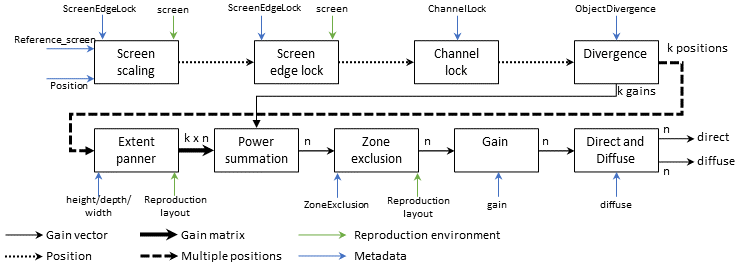
\includegraphics[width = \textwidth]{figures/ObjectPannerSignalFlow.png}
    \caption{The processing logic for calculating direct and diffuse gains for the Polar path}
    \label{fig:adm_object_polar}
\end{figure}

The first processing stage relates to whether or not the position of the Object is to be modified.
If a reproduction screen has been specified then the Object metadata can request the position of the Object be modified based on the screen properties, potentially modifying the position of the Object.
Following that, it is also possible to ensure that the object is sent only to a single loudspeaker, if one is close enough.
This is known as Channel Locking.
If no loudspeaker is within range then the Object stream is panned using its position.

Once the position of the Object has been determined, ObjectDivergence can be applied.
If the metadata specifies that Divergence be used then two additional positions are added to the Object position.
These positions are to the left and right of the Object position and their distance is specified in the metadata.
Each of these positions also has a specified gain based on the amount of divergence.
For zero divergence the original Object direction has a gain of unity and the others have zero gain.
For full divergence the original Object direction has zero gain and the left and right positions have gains of 0.5.

Once the divergence processing is complete the up-to-three divergence positions are each used to calculate a corresponding vector of panning gains based on their positions.
The gains are calculated using \code{SpreadPanner}, which allows for an azimuthal width and elevational height to be specified in the metadata.
The spread panner essentially pans copies of the Object to a set of grid positions that cover the full sphere.
A weight between 0 and 1 is applied to each of these grid positions based on the metadata width and height parameters before normalisation of the total weight by the sum of the grid weights.
The larger the width and height of the specified spread, the more of the grid points have non-zero gains, leading to a larger source width.
Each grid point then has panning gains calculated using vector base amplitude panning (VBAP) \cite{Pulkki1997} based on their position.
These gains are multiplied by their corresponding weights and summed to get the final panning gains for each of the three divergence positions.
Each of these three vectors of gains are summed using the divergence gains and they are power-normalised.

If ZoneExclusion is specified in the metadata then any loudspeaker in the excluded zone will have their gains shared out among other groups of loudspeakers.
The full method for calculating the downmixing matrix is given in section 7.3.12.2 of \cite{ITU2127}.

A global gain is applied to the spatialisation gains before calculation of direct and diffuse gain vectors.
The direct and diffuse gain vectors are generated by multiplying the spatialisation gains by $\sqrt{1-d}$ and $\sqrt{d}$ respectively, where $d$ is the diffuseness parameter specified in the metadata.
The Object signal is then multiplied by the direct and diffuse gain vectors.
The diffuse signal has a set of decorrelation filters of length $N$ applied to each channel, creating a less well localisable signal.
After appropriate compensation delay of $(N-1)/2$ samples is applied to the direct signal the direct and diffuse signals are summed.

\subsubsection{Cartesian Processing Path}

If the Cartesian flag is set to true then the cartesian processing path is used to render the stream.
\Cref{fig:adm_object_cartesian} shows the processing logic for the calculation of the direct and diffuse gains in \code{GainCalculator}.

\begin{figure}
    \centering
    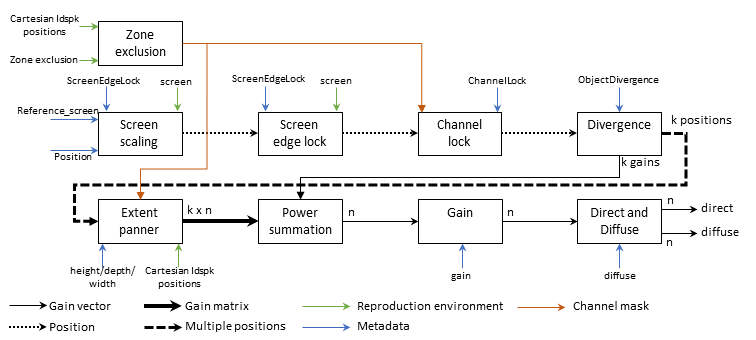
\includegraphics[width = \textwidth]{figures/ObjectPannerSignalFlowCartesian.png}
    \caption{The processing logic for calculating direct and diffuse gains for the Polar path}
    \label{fig:adm_object_cartesian}
\end{figure}

First the zone exclusion metadata is used to create a vector of masks for the loudspeakers in the reproduction layout.
These are used when calculating channel locking and extent panning later in the path.

Like the Polar path, the position of the Object is modified using screen scaling, screen edge lock and channel locking.
The channel mask from the zone exclusion is used to ensure that the object is not locked to a channel that has been excluded.

Once the position of the Object has been modified ObjectDivergence is applied.
This can create additional copies of the object panned to the left and right of its position.

For each of the divergence positions a set of loudspeaker gains is calculated using the \code{AllocentricExtent}, which uses the height, width and depth metadata parameters.
The panning uses the Cartesian/Allocentric panner rather than the PointSourcePanner of the Polar path.

These gain vectors are multiplied by their corresponding divergence gains and summed to get the final panning gains for the Object.
They are then power normalised and a gain is applied based on the metadata parameter.

Finally, the direct and diffuse gains are calculated in the same manner as for the Polar path.

\subsection{Code Example}

This example simulated receiving a mono Object stream and its meta data.
As written here, the object is rendered on a 5.1 layout at an angle of 20\deg. Try adjusting the channel locking, divergence and width to see the effect on the rendering.
For example, increasing the channel lock distance will cause the signal to snap to the left speaker completely.

\begin{lstlisting}[language=C++]
#include "AdmRenderer.h"

using namespace spaudio;

const unsigned int sampleRate = 48000;
const int nBlockLength = 512;

// Ambisonic order (not used in this example but expected in Configure())
const unsigned int nOrder = 1;

std::vector<float> sinewave(nBlockLength);
// Fill the vector with a sine wave
for (int i = 0; i < nBlockLength; ++i)
    sinewave[i] = (float)std::sin((float)M_PI * 2.f * 440.f * (float)i / (float)sampleRate);

// Prepare the stream to hold the rendered audio (5.1)
const unsigned int nLdspk = 6;
float** renderStream = new float* [nLdspk];
for (unsigned int i = 0; i < nLdspk; ++i)
{
    renderStream[i] = new float[nBlockLength];
}

// Prepare the metadata for the stream
ObjectMetadata objectMetadata;
objectMetadata.trackInd = 0;
objectMetadata.blockLength = nBlockLength;
objectMetadata.cartesian = false;
objectMetadata.position.polarPosition().azimuth = 20.;
objectMetadata.position.polarPosition().elevation = 0.;
objectMetadata.position.polarPosition().distance = 1.;

// Channel lock (off by default)
objectMetadata.channelLock = ChannelLock();
objectMetadata.channelLock->maxDistance = 0.f; // <- Increase this to see the signal snap to fully in the left loudspeaker

// Object divergence (off by default)
objectMetadata.objectDivergence = ObjectDivergence();
objectMetadata.objectDivergence->azimuthRange = 30.; // <- Controls the width of the divergence
objectMetadata.objectDivergence->value = 0.; // <- Increase this to apply object divergence

// Object extent (off by default)
objectMetadata.width = 0.; // <- Increase this to increase the width and spread the Object over more adjacent loudspeakers

// Configure the stream information. In this case there is only a single channel stream
StreamInformation streamInfo;
streamInfo.nChannels = 1;
streamInfo.typeDefinition.push_back(TypeDefinition::Objects);

// Set up the Renderer
Renderer renderer;
renderer.Configure(OutputLayout::FivePointOne, nOrder, sampleRate, nBlockLength, streamInfo);

// Add the Object stream to be rendered
renderer.AddObject(sinewave.data(), nBlockLength, objectMetadata);

// Render the stream
renderer.GetRenderedAudio(renderStream, nBlockLength);

// Cleanup
for (unsigned i = 0; i < nLdspk; ++i)
    delete[] renderStream[i];
delete[] renderStream;
\end{lstlisting}

\section{ADM HOA Rendering}\label{AdmHOA}

\subsection{Overview}

\code{Renderer} allows for Higher Order Ambisonics (HOA) streams to be decoded to any of the specified loudspeaker layouts.
It supports decoding up to a maximum of order 3.
Decoding is performed using the AllRAD method, using the \code{AmbisonicAllRAD} class internally. See \cref{AmbiDecoding} for more details about the AllRAD method.

The HOA stream has the "order" and "degree" of each channel defined in its metadata which is used to sort the channels of the stream.
\code{Renderer} uses the ACN channel sorting internally.

The normalisation of the orders can be SN3D, N3D or FuMa.
The signals are converted to SN3D, if they are not already.

Converting to ACN channel sorting and SN3D normalisation ensures the signal is in the AmbiX format, ensuring the signals are compatible with the \libspataud Ambisonics processors.

Full details can be found in section 9 of Rec. ITU-R BS.2127-1 \cite{ITU2127}.

\subsection{Code Example}

In this example an HOA signal is decoded to binaural. The AmbiX (SN3D/ACN) HOA stream and its metadata are generated as part of the example but would normally be received from the stream to be rendered.

The HOA stream is then added to the renderer using \code{AddHOA()}, which adds it to an internal buffer. \code{AddHOA()} can be called multiple times if there are multiple HOA streams to be rendered. When \code{GetRenderedAudio()} is called the accumulated HOA buffer is decoded to the specified output format. The internal HOA buffer is then cleared so that new streams can be added to the next frame to be rendered.

For a more complete example with multiple different stream types being rendered see \cref{AdmFullCodeExample}.

\begin{lstlisting}[language=C++]
#include "AdmRenderer.h"

using namespace spaudio;

const unsigned int sampleRate = 48000;
const int nBlockLength = 512;

// Higher ambisonic order means higher spatial resolution and more channels required
const unsigned int nOrder = 1;
const unsigned int nHoaCh = OrderToComponents(nOrder, true);
// Set the fade time to the length of one block
const float fadeTimeInMilliSec = 1000.f * (float)nBlockLength / (float)sampleRate;

std::vector<float> sinewave(nBlockLength);
// Fill the vector with a sine wave
for (int i = 0; i < nBlockLength; ++i)
    sinewave[i] = (float)std::sin((float)M_PI * 2.f * 440.f * (float)i / (float)sampleRate);

// Destination B-format buffer
BFormat myBFormat;
myBFormat.Configure(nOrder, true, nBlockLength);
myBFormat.Reset();

// Set up and configure the Ambisonics encoder
AmbisonicEncoder myEncoder;
myEncoder.Configure(nOrder, true, sampleRate, fadeTimeInMilliSec);

// Set test signal's initial direction in the sound field
PolarPosition<float> position;
position.azimuth = 0.5f * (float)M_PI;
position.elevation = 0;
position.distance = 1.f;
myEncoder.SetPosition(position);
myEncoder.Reset();
myEncoder.Process(sinewave.data(), nBlockLength, &myBFormat);

// Prepare the stream to be processed by the renderer
float** hoaStream = new float* [nHoaCh];
for (unsigned int i = 0; i < nHoaCh; ++i)
{
    hoaStream[i] = new float[nBlockLength];
    myBFormat.ExtractStream(hoaStream[i], i, nBlockLength);
}

// Prepare the stream to hold the rendered audio (binaural)
float** renderStream = new float* [2];
for (unsigned int i = 0; i < 2; ++i)
{
    renderStream[i] = new float[nBlockLength];
}

// Prepare the metadata for the stream
HoaMetadata hoaMetadata;
hoaMetadata.normalization = "SN3D";

// Configure the stream information. In this case there is only a single HOA stream of (nOrder + 1)^2 channels
StreamInformation streamInfo;
for (unsigned int i = 0; i < nHoaCh; ++i)
{
    streamInfo.nChannels++;
    streamInfo.typeDefinition.push_back(TypeDefinition::HOA);

    // Set the metadata for each channel
    int order, degree;
    ComponentToOrderAndDegree(i, true, order, degree);
    hoaMetadata.degrees.push_back(degree);
    hoaMetadata.orders.push_back(order);
    hoaMetadata.trackInds.push_back(i);
}

// Set up the Renderer
Renderer renderer;
renderer.Configure(OutputLayout::Binaural, nOrder, sampleRate, nBlockLength, streamInfo);

// Add the HOA stream to be rendered
renderer.AddHoa(hoaStream, nBlockLength, hoaMetadata);

// Render the stream
renderer.GetRenderedAudio(renderStream, nBlockLength);

// Cleanup
for (unsigned i = 0; i < nHoaCh; ++i)
    delete[] hoaStream[i];
delete[] hoaStream;
for (unsigned i = 0; i < 2; ++i)
    delete[] renderStream[i];
delete[] renderStream;
\end{lstlisting}

\section{ADM DirectSpeaker Rendering}\label{AdmDirectSpeaker}

\subsection{Overview}

A mono audio stream with DirectSpeaker metadata is spatialised by sending it directly to the specified loudspeaker i.e. a DirectSpeaker stream labelled as belonging to the left loudspeaker will be sent to it directly.
If the specified loudspeaker is not present in the reproduction layout then it checks a set of MappingRules.
In the case a suitable mapping rule exists, it will be used to calculate the gains to be applied to the stream.

As a fallback, or if no label is supplied, the position of the DirectSpeaker stream can be specified.
After screen edge locking, the position of the stream is checked and if there is a sufficiently close loudspeaker then the signal will be sent directly to it.
If no loudspeaker is close enough then the DirectSpeaker stream is panned as a point source to its specified direction.

Full details can be found in section 8 of Rec. ITU-R BS.2127-1 \cite{ITU2127}.

\subsection{Code Example}

In this example a DirectSpeaker signal for the wide-left (M+060) loudspeaker from a 9+10+3 layout is rendered to a 5.1 layout. The stream and its metadata are generated as part of the example but would normally be received from the stream to be rendered.

The stream is first added to be rendered using \code{AddDirectSpeaker()}. When \code{GetRenderedAudio()} is called the stream is converted (in this case) to binaural and the DirectSpeaker buffer internally is cleared, ready for the next \code{AddDirectSpeaker()} call.

\begin{lstlisting}[language=C++]
#include "AdmRenderer.h"

using namespace spaudio;

const unsigned int sampleRate = 48000;
const int nBlockLength = 512;

// Ambisonic order (not used in this example but expected in Configure())
const unsigned int nOrder = 1;

std::vector<float> sinewave(nBlockLength);
// Fill the vector with a sine wave
for (int i = 0; i < nBlockLength; ++i)
    sinewave[i] = (float)std::sin((float)M_PI * 2.f * 440.f * (float)i / (float)sampleRate);

// Prepare the stream to hold the rendered audio (5.1)
const unsigned int nLdspk = 6;
float** renderStream = new float* [nLdspk];
for (unsigned int i = 0; i < nLdspk; ++i)
{
    renderStream[i] = new float[nBlockLength];
}

// Prepare the metadata for the stream
DirectSpeakerMetadata directSpeakerMetadata;
directSpeakerMetadata.trackInd = 0;
directSpeakerMetadata.speakerLabel = "M+060"; // Wide-left speaker
directSpeakerMetadata.audioPackFormatID = std::string("AP_00010009"); // 9+10+3 layout

// Configure the stream information. In this case there is only a single channel stream
StreamInformation streamInfo;
streamInfo.nChannels = 1;
streamInfo.typeDefinition.push_back(TypeDefinition::DirectSpeakers);

// Set up the Renderer
Renderer renderer;
renderer.Configure(OutputLayout::FivePointOne, nOrder, sampleRate, nBlockLength, streamInfo);

// Add the DirectSpeaker stream to be rendered
renderer.AddDirectSpeaker(sinewave.data(), nBlockLength, directSpeakerMetadata);

// Render the stream
renderer.GetRenderedAudio(renderStream, nBlockLength);

// Cleanup
for (unsigned i = 0; i < nLdspk; ++i)
    delete[] renderStream[i];
delete[] renderStream;
\end{lstlisting}

\section{Binaural Rendering}\label{AdmBinaural}

\subsection{Overview}

The ADM specification does not have a specific implementation for rendering to binaural. EBU's BEAR \cite{EBU3369} provides a method for rendering an ADM stream to binaural.
However, BEAR requires a  binaural room impulse responses (BRIRs) that would increase the size of \libspataud by too large a degree.

Therefore, the binaural rendering of \code{Renderer} is inspired by BEAR in its use of a virtual loudspeaker layout but the final binauralisation is performed differently, in order to remove the requirement for including more HRTFs than those used for \code{AmbisonicBinaurlization}.

BEAR uses a virtual 9+10+5 loudspeaker layout and then binauralises the loudspeaker signals using BRIRs in the corresponding directions based on the loudspeaker position and the listener head orientation.

\code{Renderer} uses the same virtual loudspeaker layout for rendering Object and DirectSpeaker signals.
These loudspeaker signals are then converted to Ambisonics by encoding them based on the loudspeaker directions (ignoring listener head rotation).
This encoded signal is then summed with any HOA streams that have been added.
The composite stream is then rotated using `AmbisonicRotator` to apply the listener head rotation.
Finally, any direct binaural signal are added to the output.
The signal flow is shown in the \cref{fig:adm_binaural}.

\begin{figure}
    \centering
    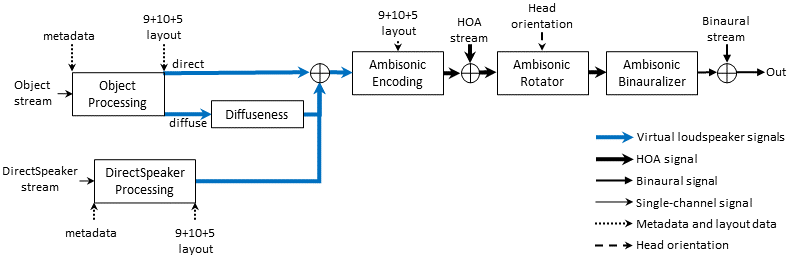
\includegraphics[width = \textwidth]{figures/AdmBinauralSignalFlow.png}
    \caption{The signal flow for the \libspataud binaural ADM renderer.}
    \label{fig:adm_binaural}
\end{figure}

\subsubsection{Advantages and Disadvantages Compared to BEAR}

The advantages of this method, besides the fact that no new HRTFs need to be added to the library, are that:
\begin{itemize}
    \item the number of expensive convolution is kept low. BEAR needs 48 convolutions (24 loudspeakers, 2 ears) to be performed, compared to 32 using the described method (16 channels, 2 ear). Furthermore, since BEAR uses BRIR the CPU load of the convolutions is increased compared to using anechoic HRIRs.
    \item custom HRTFs can be easily loaded using the .SOFA file format.
    \item in case very low CPU use is required the binaural rendering can use 1st order Ambisonics internally, reducing the number of convolutions to only 8 (or 4 if the symmetric head assumption is used).
\end{itemize}

The main disadvantage of this method is that the lack of the room in rendered binaural could reduce externalisation when compared to the BRIR method. It has been shown that using a BRIR instead of an anechoic HRIR can improve externalisation.

\subsection{Code Example}

See \cref{AdmFullCodeExample} in the main ADM overview for a full code example that renderers multiple different stream types to binaural.

\medskip

\bibliography{biblio}

\end{document}
t}
}
